\documentclass[10pt]{article}
\usepackage{multicol}
\usepackage{amsmath}
\usepackage{graphicx}
\usepackage{amsfonts}
\usepackage{amsthm}
%\usepackage{cite}
\usepackage{times}
\usepackage{geometry}
\usepackage[round,numbers,sort&compress]{natbib}
\oddsidemargin=0.0in %%this makes the odd side margin go to the default of 1inch
\evensidemargin=0.0in
\textwidth=6.5in
\textheight=9in %%sets the textwidth to 6.5, which leaves 1 for the remaining right margin with 8 1/2X11inch paper

\providecommand{\ve}[1]{\boldsymbol{#1}}
\providecommand{\norm}[1]{\left \lVert#1 \right  \rVert}
\providecommand{\deter}[1]{\lvert #1 \rvert}
\providecommand{\abs}[1]{\lvert #1 \rvert}
\providecommand{\tran}{\mbox{${}^{\text{T}}$}}
\providecommand{\transpose}{\mbox{${}^{\text{T}}$}}
\providecommand{\ve}[1]{\boldsymbol{#1}}
\DeclareMathOperator*{\argmax}{argmax}
\DeclareMathOperator*{\argmin}{argmin}
\DeclareMathOperator*{\find}{find}

\newcommand{\thetn}{\ve{\theta}}
\newcommand{\theth}{\widehat{\ve{\theta}}}
\newcommand{\theto}{\ve{\theta}'}
\newcommand{\p}{P_{\thetn}}
\newcommand{\phat}{\widehat{P}_{\thetn}(F_v | \Ca_t)}
\newcommand{\pT}{P_{\thetn_{Tr}}} %\thetn_T
\newcommand{\pO}{P_{\thetn_o}} %\thetn_o
\newcommand{\Q}{Q(\thetn,\theto)}
\newcommand{\m}{m^{\ast}}
\newcommand{\q}{q\big(\ve{H}_t^{(i)}\big)}
\newcommand{\Ca}{[\text{Ca}^{2+}]}
\newcommand{\wCab}{[\widehat{\text{Ca}}^{2+}]_b}

%\usepackage[hypertex]{hyperref}    %for LaTeX
\usepackage{hyperref}               %for pdfLaTeX

\title{Spike inference from calcium imaging using sequential Monte Carlo methods}%Model based optimal inference of spike times and calcium transients given calcium sensitive fluorescence observations}

\author{Joshua T. Vogelstein$^\ast$, Brendon O. Watson$^{\#\S}$,  Adam M. Packer$^{\#\S}$, \\ Rafael Yuste$^{\#\S}$, Bruno Jedynak$^{||}$ and Liam Paninski$^\P$ \\  $^\ast$ Department of Neuroscience, Johns Hopkins School of Medicine \\ $^\#$ Department of Biological Sciences, Columbia University \\ $^\S$ Howard Hughes Medical Institute, \\
$^{||}$ Department of Applied Mathematics and Statistics, Johns Hopkins University \\
$^\P$Department of Statistics and Center for Theoretical Neuroscience, Columbia University}

\begin{document}
\maketitle
\begin{abstract}

As recent advances in calcium sensing technologies facilitate simultaneously imaging action potentials in neuronal populations, complementary analytical tools must also be developed to maximize the utility of this experimental paradigm. While the observations here are fluorescence movies, the signals of interest --- spike trains and/or time varying intracellular calcium concentrations --- are hidden.  Inferring these hidden signals is often problematic due to noise, nonlinearities, slow imaging rate, and unknown biophysical parameters. We overcome these difficulties by developing sequential Monte Carlo methods (particle filters) based on biophysical models of spiking, calcium dynamics, and fluorescence. We show that even in simple cases, the particle filters outperform the optimal linear (i.e., Wiener) filter, both by obtaining better estimates and by providing errorbars. We then relax a number of our model assumptions to incorporate nonlinear saturation of the fluorescence signal, as well external stimulus and spike history dependence (e.g., refractoriness) of the spike trains. Using both simulations and in vitro fluorescence observations, we demonstrate temporal superresolution by inferring when within a frame each spike occurs. Furthermore, the model parameters may be estimated using expectation maximization with only a very limited amount of data (e.g. $\sim 5-10$ s or $5-40$ spikes), without the requirement of any simultaneous electrophysiology or imaging experiments.

\emph{Key words:} two photon; nonlinear deconvolution; fluorescent protein; calcium dye; fluorescent protein; generalized linear model 

\emph{Corresponding author}: Joshua Vogelstein, joshuav@jhu.edu

\end{abstract}

\newpage
\pagestyle{myheadings}
\markright{Spike times from fluorescence movies}


%\begin{multicols}
\section*{Introduction}
\addcontentsline{toc}{section}{Introduction}

Recently, advances in the development of calcium indicators, delivery techniques, and microscopy technologies have facilitated imaging a wide array of preparations \cite{ImagingManual}. In particular,  calcium sensitive organic dyes \cite{Tsien81, YusteKatz91} have been targeted to populations of neurons both in vivo and in vitro using bulk loading  \cite{YusteKatz91, BrusteinKonnerth03, StosiekKonnerth03} and electroporation  \cite{NagayamaChen07, NevianHelmchen07}.  Similarly, viral infection, transgenics, and knock-ins have been used to genetically target neurons with fluorescent proteins \cite{MiyawakiTsien97, GriesbeckTsien01, NakaiImoto01%, ShanerTsien04, GuerreroIsacoff05, OhkuraNakai05
} . In conjunction with the development of improved calcium indicators and loading techniques, the advent of 2-photon microscopy now enables the visualization of neurons deep within scattering tissue \cite{DenkWebb90, OheimCharpak01, TheerDenk03, FlusbergSchnitzer05a}.

Thus, using calcium sensitive fluorescence to study neural dynamics is becoming increasingly popular in a wide variety of neural substrates, including individual spines \cite{MullerConnor91, YusteDenk95, EngertBonhoeffer99, NimchinskySvoboda04}, dendrites \cite{MajewskaYuste00, ScheussSvoboda06, SdrullaLinden07}, boutons \cite{MajewskaSur06, BrenowitzRegehr07}, neurons \cite{HelmchenSakmann96, SvobodaDenk96, MaravallSvoboda00}, and populations of neurons \cite{YusteKatz91, O'MalleyFetcho96, SmettersYuste99, IkegayaYuste04, NiellSmith05, OhkiReid05, OhkiReid06, YaksiFriedrich07, NagayamaChen07, SatoSvoboda07, RootWang07}. While the data collected from these experiments are fluorescence movies, the signals of interest are the precise spike times and/or the intracellular calcium concentrations, $\Ca$, of the observable neurons.

Inferring the spike trains and calcium concentrations from a fluorescence signal, however, is a difficult problem for a number of reasons.  First, observations are noisy.  This is a problem unlikely to be solved in the near future, as a major noise source is photon shot noise \cite{SjulsonMiesenbock07}, which reflects the quantal nature of light emission and detection. Second, observations may have poor temporal resolution.  While this problem may be partially mitigated by faster cameras and scanning systems \cite{FlusbergSchnitzer05a,FanEllisman99, NguyenParker01, IyerSaggau06}, faster imaging tends to exacerbate the noise problem, as fewer photons can be collected per image frame \cite{SjulsonMiesenbock07}.  Third, the relationship between fluorescence observations and $\Ca$ is nonlinear, especially for fluorescent proteins \cite{PologrutoSvoboda04, TayYue07}.  This has placed undesirable and unnecessary restrictions on the calcium indicators used for analysis, as the standard analytical tools assume a linear relationship between $\Ca$ and fluorescence \cite{YasudaSvoboda04, ReiffBorst05, YaksiFriedrich06, SjulsonMiesenbock07} (though see \cite{BorstAbarbanel07} for an exception). Fourth, the parameters governing the calcium and fluorescence dynamics are typically unknown a priori, and must be inferred from the data.

Nevertheless, there has been some significant recent progress.  For instance, Smetters et al.  \cite{SmettersYuste99} demonstrated reliable detection of  single action potentials and spike trains by imaging bulk loaded fluorescent calcium dyes in vitro. Kerr et al. \cite{KerrHelmchen05} --- motivated by the observation that neurons in the rat motor and somatosensory cortices exhibit sparse spiking --- developed a custom template-matching algorithm to detect the presence of single spikes in vivo using only fluorescence signals (and more recently further refined this approach \cite{GreenbergKerr08}).  The following year, Yaksi and Friedrich  \cite{YaksiFriedrich06} --- aided by the observation that neurons in the intact zebrafish olfactory bulb tend to respond to different odors with different time-varying firing rates --- developed a linear smoothing convolution kernel that effectively inferred the time varying firing rate for an explant of an intact zebrafish brain.  More recently, Sato et al.  \cite{SatoSvoboda07} designed a clustering algorithm using only in vivo calcium sensitive fluorescence signals to determine whether whisker stimulation successfully induced a spike. Earlier this year, Holekamp et al. \cite{HolekampHoly08} applied the optimal linear filter for deconvolving a fluorescence signal from anesthetized mice. Finally, Sasaki et al. developed a nonparametric approach to infer spikes from somatic calcium fluctuations \cite{SasakiIkegaya08}. 

The present work differs from previous efforts in several key aspects.  We start by constructing a well defined probabilistic ``forward model'' of the signals of interest and the imaging process.  Then, utilizing a sequential Monte Carlo expectation maximization framework, we design a particle filter smoother (PFS) to optimally infer the spike times and calcium transients, given the observed fluorescence signals and the model. Even for relatively simple scenarios, the PFS outperforms optimal linear deconvolution by providing both a better inference and errorbars. The forward model may be generalized to account for a number of features present in typical data sets. Specifically, by incorporating saturation and signal dependent noise sources, we can perform inference on typical in vitro data sets.  Furthermore, by allowing for intermittent observations (typical of 2-photon scanning experiments), we can perform superresolution inference, i.e., detect not just whether a spike occurs within a particular image frame, but also when within that frame the spike occurred. By also introducing stimulus and spike history dependence into the model, we can further refine our estimate. Moreover, estimating the parameters requires only a few seconds of fluorescence observations and a small number of spikes (e.g., $5-40$), and does not require tedious simultaneous electrophysiology and imaging experiments. We close by discussing further generalizations of the model that may be required to apply a PFS to other experimental preparations, such as in vivo imaging. All code is available from the corresponding author upon request.

\section*{Model} \label{sec:model}
\addcontentsline{toc}{section}{Model}

The data sets of interest are sequences of images corresponding to the calcium sensitive fluorescence signals of some neural activity. We aim here to construct the simplest forward model that permits one to satisfactorily infer the spike trains and calcium transients underlying these images. By forward model, we mean a complete characterization of the probability distributions governing the hidden dynamics and noisy observations, going ``forward'' from the spike train to the images. To infer the spike trains from the observations, we then invert our model. Below, we introduce a very simple model used to explain the mathematical formalism developed to infer the spike trains. Many of the simplifying assumptions are then relaxed in the Results section to improve our estimates when using in vitro data.  %The Discussion section describes further relaxations that may be necessary for other experimental settings (e.g., in vivo).  

First,we assume a single-compartmental, equipotential model of the imaged neuron, over which the fluorescence signal may be spatially averaged, yielding a one-dimensional time varying fluorescence signal for each image frame, $F_t$.  This assumption is justified by the observation that the calcium dynamics within the neuron are relatively fast \cite{SabatiniRegehr98, MajewskaYuste00}. Next, we assume that the fluorescence at any time is a noisy linear function of $\Ca$ at that time:

\begin{align} \label{eq:F_t}
F_t &= \alpha \Ca_t + \beta + \sigma_F \varepsilon_{F,t},% \qquad \varepsilon_{F,t} \sim \mathcal{N}(\varepsilon_t; 0,1),
\end{align}

\noindent where $\alpha$ and $\beta$ set the scale and offset for the fluorescence signal, respectively, $\sigma_F$ is the standard deviation of the noise, and  $\varepsilon_{\cdot,t}$ denotes a standard normal Gaussian throughout this text. % (and $x \sim \mathcal{N}(x; \mu,\sigma^2)$ indicates that $x$ has a Gaussian distribution with mean $\mu$ and variance $\sigma^2$). %throughout this text $\varepsilon_t$ indicates a standard normal random variable (i.e., a Gaussian with mean zero and variance one), sampled independently at each time step. Note that the noise can be assumed to be a standard normal because the mean and variance would not be identifiable, as they could be scaled by $\alpha$ and $\beta$ without loss of generality.  

Modeling $\Ca_t$ requires some additional assumptions. First, after each spike, $\Ca_t$ jumps instantaneously. This approximation is justified by the observation that calcium rise time is quick relative to the decay time \cite{YasudaSvoboda04, CornelisseMansvelder07}. Second, each jump is the same size, $A$; that is, for now we neglect $\Ca_t$ saturation effects due to channel inactivation and buffering \cite{RegehrAtluri95}. Third, $\Ca_t$ decays exponentially with time constant $\tau$, to a baseline calcium concentration, $\Ca_b$; i.e., we lump the myriad calcium extrusion and endogenous buffering mechanisms and assume a single average time constant. Fourth, the $\Ca_t$ dynamics themselves have some Gaussian noise source, scaled by $\sigma_c$. Taken together, these assumptions imply the following model:

\begin{multline} \label{eq:C_t}
\Ca_t - \Ca_{t-1} =\\ -\frac{\Delta}{\tau}(\Ca_{t-1}-\Ca_b) + A n_t + \sigma_c \sqrt{\Delta} \varepsilon_{c,t},% \qquad \varepsilon_t \mathcal{N}(\varepsilon_t; 0, \sigma_c^2 \Delta
\end{multline}

\noindent where $\Delta=1/$(frame rate) is the time step size (the variance is scaled by $\Delta$ to ensure that the noise statistics are independent of the frame rate), $n_t$ is the number of spikes that occurred in the $t$-th frame, and $\sigma_c$ scales the noise. Note that because we have assumed here a linear observation model (i.e., Eq. \ref{eq:F_t} states that $F_t$ is a linear function of $\Ca_t$), our model is overparameterized. More precisely, both $A$ and $\alpha$ set the scale, and $\Ca_b$ and $\beta$ set the offset. Furthermore, because the noise is not signal dependent, both $\sigma_F^2$ and $\alpha$ set the effective signal-to-noise ratio (SNR).  Therefore, in the following, we let $\alpha=1$, $\beta=0$, and $\sigma_F^2=1$, without loss of generality (later, we deal with this overparameterization by introducing a nonlinear observation model). 

To model the spike train, we let $n_t$ be a Bernoulli (binary) random variable, which spikes in each time step with probability $p \Delta$:

\begin{align} \label{eq:n_t}
n_t \sim \mathcal{B}(n_t; p \Delta),
\end{align}

\noindent where $\mathcal{B}(n_t;p \Delta)$ indicates that $n_t=1$ with probability $p \Delta$, and $n_t=0$ with probability $1-p \Delta$ (where $0 <p \Delta < 1$). Eq. \ref{eq:n_t} therefore implies that spiking at time $t$ is independent of other spikes and the intracellular calcium concentration. Fig. \ref{fig:noisy} depicts a spike train (top panel), the resulting calcium transients (second panel), and the fluorescence observations (third panel), simulated according to this model.

\section*{Mathematical Methods} \label{sec:math_meth}
\addcontentsline{toc}{section}{Mathematical Methods}

Given the above model, our goal is to take the entire sequence of fluorescence observations, $F_{1:T}=[F_1, \ldots, F_T]$ (where $T$ indexes the final observation in the sequence%, and we have used the notation $F_{1:T}=F_1, \ldots, F_T$
), and infer the underlying spike train, $n_{1:T}$. More formally, we want to find $\p(n_t | F_{1:T})$, the probability of the neuron spiking in each frame (which depends on the parameters, $\ve{\theta}=\{\tau, \Ca_b, A, \sigma_c, p\}$), given all the fluorescence observations.   
%Typically, one proceeds as follows:
%
%\begin{align} \label{eq:goal}
%\widehat{n_t} &= \argmax_{n_t \in \{0,1\}} \p (n_t | F_{1:T})% \nonumber \\
%= \argmax_{n_t \in \{0,1\}} \frac{\p(F_{1:T} | n_t) \p (n_t)}{\p(F_{1:T})}
%= \argmax_{n_t \in \{0,1\}} \p(F_{1:T} | n_t) \p(n_t),
%\end{align}
%
%\noindent where the second equality follows from applying Bayes rule a couple of times, and the third equality follows from the fact that $\p(F_{1:T})$ simply scales the result. Note that because these distributions are governed by a set of parameters, $\ve{\theta}$, which are typically unknown, we also provide details for finding their maximum likelihood estimators, $\widehat{\ve{\theta}}$.    
%
%Sadly, exactly solving Eq. \ref{eq:goal} requires searching over all possible spike trains, which comprise a set of size $2^T$; thus, for large $T$, this is computationally infeasible. Therefore, we instead sample $n_t$ at each time step, to construct an approximation to the above distributions.  The accuracy of this approximation is therefore highly dependent on the sampling details.  Fortunately, 
We use a framework referred to as sequential Monte Carlo (using a PFS) to find these probabilities \cite{DoucetGordon01}, embedded within an expectation maximization algorithm \cite{DempsterRubin77} to estimate the parameters. As this approach is becoming relatively common within neuroscience \cite{GaoDonoghue02, BrockwellKass04, KellyLee04, SamejimaKimura04, HuysPaninski06b, Sanger07, ErgunBrown07} --- and it may be thought of as a generalization of either (i) the Baum-Welch algorithm for Hidden Markov Models \cite{Rabiner89}, or (ii) the Kalman filter smoother for state-space models \cite{Kalman60} ---  we relegate the details to the Appendices, and simply state the general procedure here.

We must first define a number of terms. Our model consists of a number of time-varying states, each governed by a set of parameters (which are constant). The states may be subdivided into \emph{observation states}, denoted by $\ve{O}_t$, and \emph{hidden states}, denoted by $\ve{H}_t$. Together, the states comprise the complete likelihood, which may be simplified, given our model assumptions, as follows \cite{Rabiner89}:

\begin{align} \label{eq:complete}
\p (\ve{O}_{1:T}, \ve{H}_{1:T}) &= \p(\ve{H}_0) \prod_{t=1}^T \p(\ve{H}_t | \ve{H}_{t-1}) \p(\ve{O}_t | \ve{H}_t),
\end{align}

\noindent where $\p(\ve{H}_0)$ is the initial distribution distribution of hidden states, $\p(\ve{O}_t | \ve{H}_t)$ is the \emph{observation distribution} and $\p(\ve{H}_t | \ve{H}_{t-1})$ is the \emph{transition distribution}. For this model, the observation state is the fluorescence measurement, $\ve{O}_t=F_t$; and the hidden states are whether or not the neuron spiked, and the magnitude of the intracellular calcium concentration, $\ve{H}_t=\{n_t,\Ca_t\}$.  We typically take the initial distribution to be baseline values, i.e., the initial calcium is $\Ca_b$ and initial value for the spike train is $0$. The observation distribution is defined for the above model as: % The observation state is governed by the \emph{observation distribution}, which is, according to the above model:

\begin{align} \label{eq:obs_dist}
\p^L(\ve{O}_t | \ve{H}_t)  &\overset{def}{=}  \p(F_t \mid  \Ca_t,n_t) =  \p(F_t \mid  \Ca_t) \nonumber \\
&= \mathcal{N}(F_t; \alpha \Ca_t + \beta ,\sigma_F^2) = \mathcal{N}(F_t; \Ca_t, 1),
\end{align} 

\noindent which follows from Eq. \ref{eq:F_t} and the discussion following (where $\overset{def}{=}$ indicates that $\p^L(\ve{O}_t | \ve{H}_t)$ is defined for this \emph{linear} model). Similarly, the transition distribution for the above model is defined as: %state is governed by the \emph{transition distribution}, which is, for the above model:

\begin{align} \label{eq:trans_dist}
\p^L(\ve{H}_t | \ve{H}_{t-1}) &\overset{def}{=} \p(\Ca_t,n_t \mid \Ca_{t-1},n_{t-1}) %\nonumber \\
%&
= \p(\Ca_t \mid \Ca_{t-1}, n_t) \p(n_t) \nonumber \\
&= 
\begin{cases}
\mathcal{N}\big(\Ca_t; \widehat{\mu}(n_t), \sigma_c^2 \Delta\big) (p \Delta)& \text{if } n_t=1 \\
\mathcal{N}\big(\Ca_t; \widehat{\mu}(n_t), \sigma_c^2 \Delta\big) (1-p \Delta)& \text{otherwise,}\\
\end{cases}
\end{align}

\noindent where $\widehat{\mu}(n_t)=\Ca_t - \Delta/\tau(\Ca_{t-1}-\Ca_b) + A n_t$, and the above equation follows from Eqs. \ref{eq:C_t} and \ref{eq:n_t}.

Now the goal is to efficiently estimate $\p(\ve{H}_t | \ve{O}_{1:T})=\p(n_t, \Ca_t \mid F_{1:T})$  for all $t$, the posterior distribution of the hidden signals, given all the observations. Estimating this distribution is problematic, because spike trains are inherently nonlinear.  Therefore, linear filters (such as the Wiener filter), are inadequate, so nonlinear filters (such as particle filters), must be employed.   We proceed by taking a particle filter-smoother (PFS) approach, which breaks this problem down into two recursions.  In the forward recursion, we recursively estimate $\p(n_t, \Ca_t \mid F_{1:t})$, the probability of spiking and $\Ca$ at time $t$, given the fluorescence observations from time $1$ up to and including $t$.  Upon reaching time $T$, we recurse backward until $t=1$, to get $\p(n_t, \Ca_t \mid  F_{1:T})$, the probability of spiking and $\Ca$ at time $t$ given \emph{all} the fluorescence observations (i.e., both before and after $t$).


We use a particle filter to approximate the forward recursion.  The key is that $\p(\ve{H}_t | \ve{O}_{1:t})$ may be well approximated by generating a number of weighted samples (or ``particles'') \cite{DoucetGordon01}:

\begin{align} \label{eq:PF}
\p(\ve{H}_t |  \ve{O}_{1:t}) \approx \sum_{i=1}^N w_t^{(i)} \delta \big( \ve{H}_t - \ve{H}_t^{(i)}\big),
\end{align}

\noindent where $w_t^{(i)}$ is the relative likelihood of the state at time $t$ taking value $\ve{H}_t^{(i)}$, and $\delta(\cdot)$ is the Dirac delta function (i.e., $\delta(x)=1$ when $x=0$ and $\delta(x)=0$ otherwise). Thus, at each time step, one samples $N$ particles, and then computes the weight of each. It can be shown that the weights may be recursively computed by using \cite{DoucetGordon01},:

\begin{align} \label{eq:WEIGHT}
w_t^{(i)} \approx  \frac{\p\big(\ve{O}_t | \ve{H}_t^{(i)}\big) \p\big(\ve{H}_t^{(i)} | \ve{H}_{t-1}^{(i)}\big) w_{t-1}^{(i)}}{\q},
\end{align}

\noindent where $\q$, the \emph{sampling distribution} (or sampler) is chosen to make the approximation in Eq. \ref{eq:PF} as accurate as possible.  In general, the sampler may depend on all the particle history and any observations (both past and future).  The most common choice is the ``prior sampler'',  $\q=\p(\ve{H}_t^{(i)} | \ve{H}_{t-1}^{(i)})$, in which we sample directly from the transition distribution. The prior sampler is very simple to use, because we know how to sample from each of the distributions comprising the transition distribution for this model  (given by Eq. \ref{eq:trans_dist}). The next most common choice is the ``one-observation-ahead sampler'' \cite{DoucetGordon01},  $\q=\p(\ve{H}_t^{(i)} | \ve{H}_{t-1}^{(i)}, \ve{O}_t)$, which may be written explicitly in terms of our model:

\begin{align} \label{eq:SAMP}
\q=\p(\ve{H}_t^{(i)} | \ve{H}_{t-1}^{(i)}, \ve{O}_t) & =
\p (n_t^{(i)},\Ca_t^{(i)} | n_{t-1}^{(i)}, \Ca_{t-1}^{(i)}, F_t)
\nonumber \\ &= \p \big( F_t \mid \Ca_t^{(i)} \big) \p \big( \Ca_t^{(i)}   \mid \Ca^{(i)}_{t-1}, n_t^{(i)} \big)  \p \big( n_t^{(i)} \big)/Z, 
\end{align}

\noindent where the equalities follow from our model assumptions, and $Z$ acts as a normalizing constant that does not depend on $\{n_t, \Ca_t\}$. The one-observation-ahead sampler conditions directly on the next fluorescence observation, and therefore ``anticipates'' where to best place the next hidden samples (see Appendix \ref{sec:cond_samp} for details). In practice, the one-observation-ahead sampler is more efficient than the prior sampler, meaning that we can use fewer particles to obtain the same accuracy for the approximation in Eq. \ref{eq:PF} \cite{DoucetGordon01}. Thus, all the particle filters developed here implement the one-observation-ahead sampler (or a close approximation to it).

%The two typical choices are the prior (or transition) sampler, $\p(\ve{H}_t^{(i)} | \ve{H}_{t-1}^{(i)})$, and the so-called ``one-observation-ahead'' sampler, $\p(\ve{H}_t^{(i)} | \ve{H}_{t-1}^{(i)}, \ve{O}_t)$ \cite{DoucetGordon01}. While the prior sampler is simpler, the one-observation-ahead sampler is more efficient, as it samples conditioned on both the previous state, $\ve{H}_{t-1}^{(i)}$, and the current observation, $\ve{O}_t$.  For the above model, the one-observation-ahead sampling distribution may be written explicitly as:
%
%\noindent which follows from Eqs. \ref{eq:obs_dist} and \ref{eq:trans_dist}, and the application of Bayes' rule several times.  This sampling distribution conditions directly on the fluorescence observation, and therefore ``anticipates'' where to best place the next hidden samples (see Appendix \ref{sec:cond_samp} for details).  

When implementing either sampler, after iterating several time steps, the weights of some of the particles approach zero, making the representation in Eq. \ref{eq:PF} degenerate, and therefore hurting the quality of the particle approximation. To remedy this situation, whenever the approximate effective number of particles drops below some threshold (typically taken to be $N/2$), the particles may be ``resampled'', by sampling (with replacement) from the population of particles.  The probability of resampling each particle is related to its weight \cite{DoucMoulines05} 
%After sampling $N$ times from Eq. \ref{eq:SAMP}, and computing the weights for each sample according to Eq. \ref{eq:WEIGHT}, we must ``resample'' the particles \cite{DoucetGordon01}.  The basic idea of resampling is to eliminate unlikely particles, and replicate very likely particles, which is performed whenever the distribution of weights yields an unsatisfactory approximation to the desired distribution.  More specifically, we can sample (with replacement) from our population of particles, where the likelihood of sampling particle $\ve{H}_t^{(i)}$ is proportional to the weight of that particle, $w_t^{(i)}$.  As resampling necessarily reduces the particle diversity, it is only performed when the variance gets too large 
(see Appendix \ref{sec:cond_samp} for details of how to weight and resample from this distribution).

One recursively repeats these three steps (sampling, computing weights, and resampling if necessary) for each time step, starting at $t=1$, and continuing through $t=T$, thus completing the forward recursion (i.e., the particle filter), and yielding an approximation to $\p(\ve{H}_t |  \ve{O}_{1:t})$ for each time step. Upon reaching $t=T$, one initializes $\p(\ve{H}_T^{(i)}|\ve{O}_{1:T})=w_T^{(i)}$, and then uses the following backward recursion, going from $t=T$ to $t=1$, to approximate $\p(\ve{H}_t | \ve{O}_{1:T})$ for each time step:

\begin{subequations} \label{eq:part_back1}
\begin{align} \label{eq:part_joint1}
\p(\ve{H}_t^{(i)}, \ve{H}_{t-1}^{(j)} | \ve{O}_{1:T}) %\\&
&=\p \big(\ve{H}^{(i)}_t | \ve{O}_{1:T}\big) \frac{
\p \big(\ve{H}^{(i)}_t | \ve{H}^{(j)}_{t-1} \big)
w_{t-1}^{(j)}}{\sum_j \p \big(\ve{H}^{(i)}_t | \ve{H}^{(j)}_{t-1} \big) w_{t-1}^{(j)}}
\\ \label{eq:part_marg1}  \p(\ve{H}_{t-1}^{(j)} | \ve{O}_{1:T})
&= \sum_{i=1}^N \p(\ve{H}_t^{(i)}, \ve{H}_{t-1}^{(j)} | \ve{O}_{1:T}).
\end{align}
\end{subequations}

\noindent This backward recursion is often referred to as a ``particle smoother'', and comprises the backward component of our PFS approach.  Thus, our PFS provides the distributions in Eq. \ref{eq:part_back1} (for a particular model).  For instance, the \emph{linear observation} particle filter provides the distributions in Eq. \ref{eq:part_back1}, when modeling the spiking, calcium, and fluorescence dynamics according to Eqs. \ref{eq:F_t} -- \ref{eq:n_t} (cf. Fig. \ref{fig:noisy}, bottom panel).  Given the distributions in Eq. \ref{eq:part_back1}, we can perform various inferences. For example, the expected number of spikes at each time step, given all the observations, may be computed by:

\begin{align}
E[n_t | F_{1:T}]=  \sum_{i=1}^N n_t^{(i)} \p(n_t^{(i)} | F_{1:T})=
\sum_{i=1}^N n_t^{(i)} \p(\ve{H}_t^{(i)} | \ve{O}_{1:T}). 
\end{align}

\noindent Other quantities of interest (such as the posterior variance, median, etc.) may be computed in a similar fashion, since we have computed the full posterior distribution, $\p(n_t | F_{1:T})$ (which, hereafter, is referred to as the posterior mean of the spike train, or simply inferred spike train). All these computations require reasonable estimates of the parameters. By using an expectation maximization approach \cite{DempsterRubin77}, we can iterate inferring the distributions of interest (e.g., $\p(n_t | F_{1:T})$), and learning the parameters.  More precisely, we optimize the following expected loglikelihood \cite{WillsNinness08}:

\begin{multline} \label{eq:m_tot}
\widehat{\ve{\theta}} = \argmax_{\ve{\theta}} \sum_{t=1}^T  \sum_{i,j=1}^N \\
\Bigg( P_{\theto} \big(\ve{H}_t^{(i)}, \ve{H}_{t-1}^{(j)} | \ve{O}_{1:T}\big)\times \ln \p\big(\ve{H}_t^{(i)} | \ve{H}_{t-1}^{(j)}\big) \\ 
+ \sum_{i=1}^N  P_{\theto} \big(\ve{H}_t^{(i)} | \ve{O}_{1:T}\big) \times \ln \p\big(\ve{O}_t | \ve{H}_t^{(i)}\big)\Bigg), 
\end{multline}

\noindent where $\ve{\theta}'$ is the estimate of the parameters from the previous iteration, i.e. those used to obtain the distributions in Eq. \ref{eq:part_back1},  which may be thought of as weights on the transition and observation log-densities. Importantly, the above loglikelihood for this model was constructed to ensure that all the parameters may be quickly estimated using standard gradient ascent techniques.  %Since the transition and observation distributions were chosen such that their likelihood functions have only a single maximum,  one can solve for all the parameters using standard gradient ascent techniques. Note, however, that while the likelihood for the complete loglikelihood is concave, the full marginal likelihood (i.e., $\p(\ve{H}_{1:T} | \ve{O}_{1:T})$, may not be. 
Details may be found in Appendix \ref{sec:mstep}.

%For instance, the parameters governing $\Ca_t$ may be found by solving:
%
%\begin{align} \label{eq:C_pa}
%\{\widehat{\tau}, \widehat{\sigma}\} &= \argmax_{\tau,\sigma >0} \sum_{t=1}^T \sum_{i,j=1}^N \p\big(\ve{H}_t^{(i)}, \ve{H}_{t-1}^{(j)} | \ve{O}_{1:T}\big) \ln \p \big(\Ca_t^{(i)} \mid \Ca_{t-1}^{(j)}, n_t^{(i)}\big),\nonumber \\
%&= \argmax_{\tau,\sigma >0} \sum_{t=1}^T \sum_{i,j=1}^N \p\big(\ve{H}_t^{(i)}, \ve{H}_{t-1}^{(j)} | \ve{O}_{1:T}\big) \\
%&\qquad \qquad  \ln \mathcal{N} \big( \Ca_t^{(i)}; \Ca_t -\frac{\Delta}{\tau} \big( \Ca_{t-1}^{(j)}-\Ca_b\big) +A n_t^{(i)}, \sigma^2 \Delta\big), 
%\end{align}
%
%\noindent where $\p\big(\ve{H}_t^{(i)}, \ve{H}_{t-1}^{(j)} | \ve{O}_{1:T}\big)$ is available from Eq. \label{eq:part_joint1}.  The solution to Eq. \ref{eq:C_pa} may be found using standard constrained convex optimization algorithms (see Appendix \ref{sec:mstep} for details on estimating all the parameters).

\section*{Experimental Methods} \label{sec:exp_meth}
\addcontentsline{toc}{section}{Experimental Methods}

\paragraph{Slice Preparation and Imaging}

All animal handling and experimentation was done according to the National Institutes of Health and local Institutional Animal Care and Use Committee guidelines. Somatosensory thalamocortical slices $400$ $\mu$m thick were prepared from C57BL/6 mice at age P14 as described \cite{MacLeanYuste05}. Neurons were filled with $50$ $\mu$M Fura $2$ pentapotassium salt (Invitrogen, Carlsbad, CA) through the recording pipette. Pipette solution contained $130$ K-methylsulfate, $2$ MgCl$_2$, $0.6$ EGTA, $10$ HEPES, $4$ ATP-Mg, and $0.3$ GTP-Tris, pH $7.2$ ($295$ mOsm).  After cells were fully loaded with dye, imaging was done by using a modified BX50-WI upright confocal microscope (Olympus, Melville, NY).  Image acquisition was performed with the C9100-12 CCD camera from Hamamatsu Photonics (Shizuoka, Japan) with arclamp illumination at $385$ nm and $510/60$ nm collection filters (Chroma, Rockingham, VT).  Images were saved and analyzed using custom software written in Matlab (Mathworks, Natick, MA).

\paragraph{Electrophysiology}

All recordings were made using the Multiclamp 700B amplifier (Molecular Devices, Sunnyvale, CA), digitized with National Instruments 6259 multichannel cards and recorded using custom software written using the LabView platform (National Instruments, Austin, TX) .  Waveforms were generated using Matlab and were given as current commands to the amplifier using the LabView and National Instruments system. The shape of the waveforms mimicked excitatory (inhibitory) synaptic inputs, with a maximal amplitude of $+70$ pA ($-70$ pA).

\section*{Results} \label{sec:results}
\addcontentsline{toc}{section}{Results}

\paragraph{Main Result}

The main result of this work is depicted in Fig. \ref{fig:noisy}, which shows a spike train, calcium concentration, and resulting fluorescence observations (first through third panels, respectively) when simulated according to the simple \emph{linear observation} model, Eqs. \ref{eq:F_t} -- \ref{eq:n_t} (where linear observation refers to the relationship between $\Ca_t$ and $F_t$). For this model, we developed a linear observation particle filter smoother (PFS), to perform optimal inference of the spike train (see Appendix \ref{sec:LOOPSI} for details).  While the optimal linear deconvolution (i.e., the Wiener filter; see \cite{HolekampHoly08} for a detailed discussion on using the Wiener filter to infer spikes from calcium imaging) performs reasonably well (fourth panel), even in this relatively simple example, the linear observation PFS (bottom panel) provides several advantages.  First, the spike train inferred by the linear observation PFS (dark blue, bottom panel) is a better estimate of the actual spike train than the estimate using the Wiener filter (red and blue, fourth panel). This follows because the Wiener filter assumes that the spike train has a Gaussian distribution, and therefore admits both partial and negative spikes, neither of which are possible in our model. Second, the PFS provides not only the probability of a spike occurring in each time bin, but also the entire distribution (from which we may compute errorbars; light blue in bottom panel). An even more fundamental advantage of the PFS framework is its generalizability. Below, we address a number of important generalizations to the model, each of which requires just a minor modification of the dynamics equations, sampling distribution, and particle filter (but the smoother remains the same). We then apply each generalization to in vitro data to demonstrate its utility.

%% insert noisy fig here

\paragraph{Saturation}

The relationship between the fluorescence signal and $\Ca_t$ is often characterized by a nonlinear saturating function, $S(\Ca_t)$:

\begin{align} \label{eq:mean_obs}
F_t = \alpha S(\Ca_t) + \beta + \eta_t.
\end{align} 

\noindent The above equation states that at any time, the \emph{expected value} of fluorescence is a nonlinear saturating function of the calcium signal.  The gain (or slope), $\alpha$, accounts for all the factors contributing to signal amplification, including the number of fluorophores in the neuron, the brightness of each fluorophore, the gain of the image acquisition system, etc.  The offset, $\beta$, accounts for any factor leading to a constant background signal, such as baseline fluorescence. The nonlinear saturation function, $S(\Ca_t)$, is often taken to be the Hill equation, i.e. $S(x)=x^n/(x^n+k_d)$, where $n$ is the Hill coefficient, and $k_d$ is the dissociation constant \cite{YasudaSvoboda04}. The variance, $\eta_t$, may be generalized similarly.  Assuming the primary noise source is photon shot noise, it would be appropriate to model noise as a Poisson process, which could be well approximated by a Gaussian distribution for large photon counts \cite{SjulsonMiesenbock07}:

\begin{align} \label{eq:var_obs}
\eta_t = \sqrt{\xi S(\Ca_t) + \sigma_F} \varepsilon_{F,t},
\end{align} 

\noindent where $\sigma_F$ scales the signal-to-noise ratio (SNR).  Note that there is no scale term for the saturated fluorescence component of the noise, as it would not be identifiable ($\alpha$, $\beta$, and $\sigma_F$ could be normalized by it without loss of generality). These assumptions change the observation distribution from Eq. \ref{eq:obs_dist} to:

\begin{align} \label{eq:nonlin}
\p^{NL}(\ve{O}_t | \ve{H}_t) %=   \p^{NL}(F_t \mid \Ca_t) 
\overset{def}{=} \mathcal{N}\big(F_t; \alpha S(\Ca_t) + \beta, \xi S(\Ca_t)+\sigma_F\big).
% \frac{1}{\sqrt{2 \pi} (S(\Ca_t^{(i)}) + \sigma_F)} \exp \left\{-\frac{1}{2}\left(\frac{F_t - \alpha S\big(\Ca_t^{(i)}\big) - \beta }{S(\Ca_t^{(i)}) + \sigma_F}\right)^2\right\},
\end{align}

\noindent To perform optimal inference on this model (i.e., Eqs. \ref{eq:C_t}, \ref{eq:n_t}, \ref{eq:mean_obs}, and \ref{eq:var_obs}), we construct a \emph{nonlinear observation} PFS (where nonlinear observation refers to the relationship between $F_t$ and $\Ca_t$ given by Eq. \ref{eq:nonlin}). The nonlinear observation PFS is different from the linear observation PFS because the observation distributions for which the two filters were designed differ, thus the one-observation-ahead sampler ($\q=\p(\ve{H}_t^{(i)} | \ve{H}_{t-1}^{(i)}, \ve{O}_t)$) changes (See Appendix \ref{sec:NOOPSI} for details). 

Fig. \ref{fig:SaturSim} shows an example of data simulated using the above model (Eqs. \ref{eq:C_t}, \ref{eq:n_t}, \ref{eq:mean_obs}, and \ref{eq:var_obs}; top three panels).  Two important differences between this model and the linear model are apparent.  First, the nonlinear saturating function, $S(\Ca_t)$,  causes the fluorescence to decay more slowly than the calcium. Thus, if one were to simply deconvolve the spike trains from the raw fluorescence observations, the estimate of  the spike train $(n_{1:T})$ and time constant $(\tau)$ would be biased.  Second, as $\Ca$ accumulates, the fluorescence transients due to a spike become smaller.  This reduces the effective SNR, obfuscating estimating the jump size, $A$. The Wiener filter (fourth panel), which cannot incorporate a nonlinearity, performs less well in this scenario than in the linear scenario.  This may be evident from the observation that peaks in the Wiener filter output become smaller and closer to the noise when the signal approaches saturation.   The nonlinear observation PFS, however, explicitly models this nonlinearity, and therefore can infer spikes very accurately even in the saturating regime (fifth panel). Furthermore, using the nonlinear observation PFS, we can reconstruct the unsaturated $\Ca_t$ (bottom panel) in addition to the spike train (when assuming Eq. \ref{eq:nonlin} accurately describes the relationship between calcium and fluorescence). This is an absolute estimate of $\Ca_t$, meaning that we infer the baseline calcium concentration and jump size in real units (as opposed to only relative units), which follows because relative changes in fluorescence correspond with absolute changes in the \emph{unsaturated} calcium concentration, due to the assumed nonlinear relationship between $F_t$ and $\Ca_t$.  

Fig. \ref{fig:BurstData} shows an example of saturating fluorescence observations recorded in vitro (top panel).  Within a burst, later spikes cause fluorescent transients that are smaller than the first few spikes.  This is evident from the Wiener filter, in which the inferred spike size becomes much smaller in large bursts (second panel).  The nonlinear observation PFS, however, accurately infers exactly one spike for each frame in which a spike occurred (third panel). Furthermore, we infer the underlying and non-saturating calcium transients (bottom panel), which is not possible using linear methods.  Fig. \ref{fig:SaturData} shows another example of a spike train recorded in vitro, but with far noisier observations and a more ``naturalistic'' spike train. As in Fig. \ref{fig:BurstData}, even though the effective SNR of the Wiener filter output deteriorates as the fluorescence signal saturates, the nonlinear observation PFS can accurately infer precise spike times.

%% insert satur fig here

\paragraph{Superresolution}

Technological limitations often impose an undesirable upper bound on the imaging frame rate.  In this context, superresolution denotes the ability to infer spike trains with more precision than the frame rate. Our assumptions may be generalized for superresolution inference by modifying the observation model. First, we reduce the time step size by a factor, $d$, such that $\Delta=1/(d \times$frame rate$)$.  Now we have two cases for the observation distribution: the case described by Eq. \ref{eq:nonlin} (which now occurs every $d$ time steps), and the ``null'' case, where  no observation occurs (and therefore, $\p(\ve{O}_t | \ve{H}_t)=1$). To perform optimal inference given this more sophisticated observation distribution, we develop a \emph{superresolution} PFS (see Appendix \ref{sec:SNOOPSI} for details).  Fig. \ref{fig:array} shows how the superresolution PFS inference precision scales with both imaging frame rate and observation noise. Importantly, the probability of spiking in each time step within an image is not uniform, but rather, tends to be higher around the actual spike time. As the noise is increased, the probabilities further spread and flatten, but still yield an accurate estimate of the total number of spikes per frame (assuming one tends to collect a large enough number of photons per pixel to be detected by the imaging system).  

One interesting result of this analysis is that imaging faster, while increasing noise and \emph{decreasing} SNR per frame \cite{SjulsonMiesenbock07}, can actually increase fidelity (i.e., effective SNR).  This may be seen by comparing panels arranged diagonally ascending to the right, which show how the inference performs upon increasing frame rate and noise proportionally.  Although the SNR per frame decreases, because more information is available about the decay, superior inference precision may be achieved. This suggests that given the option, it is always advantageous to image as quickly as possible, even at the expense of reduced SNR per frame.

\paragraph{Spike History and Stimulus Dependence}

So far, we have assumed that our neuron generates spikes independent of both external stimuli and its own spike history (cf. Eq. \ref{eq:n_t}). These two inputs (stimuli and spike histories) may be incorporated into this framework by replacing $p$ of Eq. \ref{eq:n_t} with a Generalized Linear Model (GLM) \cite{McCullaghNelder89}.  GLMs have recently been used extensively to model spike trains from a variety of different preparations and modalities (see, for example,  \cite{PaninskiLewi07}). While many GLMs could be applied here, to fit within the sequential Monte Carlo expectation maximization framework, we require that: (i) the loglikelihood is concave in the parameters of the GLM, and (ii) the dynamics are Markovian.  To satisfy our first constraint (concavity), we propose to allow the probability of spiking, $p_t$, to be a time-varying nonlinear function of the input to the neuron, $y_t$:

\begin{align} \label{eq:p_t}
p_t &= 1 - e^{-f(y_t) \Delta},
\end{align}

%modifying the distribution governing spiking activity. For instance, the neuron may linearly filter some multi-dimensional time-varying external stimulus.  The probability of the neuron spiking at each time may be some nonlinear function of the one-dimensional output of that filter, $y_t$:   

\noindent where $f(\cdot)$ is some convex and log-concave function (see \cite{EscolaPaninski07} for more details on Eq. \ref{eq:p_t}).  In general, the input to the neuron, $y_t$, may be subdivided into a multidimensional stimulus, $\ve{x}_t$, and a set of spike history terms, $\ve{h}_t=\{h_{1,t}, \ldots, h_{L,t}\}$, yielding:

\begin{align} \label{eq:y_t}
y_t = \ve{k}' \ve{x}_t + \ve{w}' \ve{h}_t,
\end{align}

\noindent where $\ve{k}$ is a linear filter operating on the stimulus (which is closely related to the spike-triggered-average of the neuron \cite{Paninski04c}), $\ve{w}$ weights the spike history terms \cite{TruccoloBrown05}, and $'$ denotes the transpose operation. To satisfy the second constraint above (Markovian dynamics), we use a set of exponentially decaying terms, each with a unique time constant: 

\begin{align} \label{eq:h_t}
h_{l,t} - h_{l,t-1} = - \frac{\Delta}{\tau_{h_l}}h_{l,t-1} + n_{t-1} + \sigma_{h_l} \sqrt{\Delta} \varepsilon_{l,t},
\end{align}

\noindent implying that after each spike, each spike history term jumps, and then decays back to zero with time constant $\tau_{h_l}$ (and each process has noise with variance $\sigma_{h_l}^2 \Delta$).  Eq. \ref{eq:h_t} is is sufficiently general to account for most spike history effects, including refractoriness, burstiness, facilitation, adaptation, and oscillations \cite{Paninski04}.  To optimally infer spikes given this more sophisticated model (i.e., Eqs. \ref{eq:C_t}, \ref{eq:mean_obs}, \ref{eq:var_obs}, and \ref{eq:p_t} -- \ref{eq:h_t}), we modify our superresolution PFS to incorporate the above GLM, yielding a GLM PFS (see Appendix \ref{sec:GOOPSI} for details).

Fig. \ref{fig:StimSim} shows a simulation using a model that incorporates saturation and signal dependent noise, as well as stimulus and spike history dependent spiking, with an unsatisfactorily slow frame rate (top six panels). Although the superresolution PFS accurately infers in which frame spikes occur (seventh panel), its superresolution abilities are limited due to saturation and low SNR.  By contrast, the GLM PFS accurately infers spike times with superresolution precision by utilizing the input and spike history dependence (bottom panel). Note that even when multiple spikes occur within a single image frame, the GLM PFS correctly infers the number of spikes, and provides a good estimate for the precise timing of each spike (see simulated data and inference between $0.5$ and $1$ sec). 

Fig. \ref{fig:real} uses in vitro data to compare the Wiener filter, superresolution PFS, and GLM PFS.  Here, a neuron under patch clamp (current clamp mode) was stimulated with a time-varying current (top panel).  The exact spike times were recorded electrophysiologically (second panel), while simultaneously imaging the fluorescence signal (third panel).  The Wiener filter (fourth panel) generates ``bumps'' near the frames in which spikes arrived, but generally fails to identify individual spike times.  

The superresolution PFS succeeds in identifying the spikes, but with limited temporal resolution (fifth panel).  By including stimulus information and spike history dependence, the GLM PFS further refines the temporal estimates beyond that of our sampling interval.  From this data set, we could achieve a temporal precision of approximately $25$ msec, even though observations were only obtained once per $100$ msec (bottom panel).  %The SOOPSI filter, however, can infer spike times more with some superresolution, even in the absence of spike history or stimulus dependence (fifth panel).  By including stimulus information, the GOOPSI filter further refines our estimate, to determine when within each frame a spike arrives, to a precision of $\sim 25$ msec, even though observations were only obtained once per $100$ msec (bottom panel).% Note that all the parameters were estimated using only this 6 s of data, containing only 19 spikes.  %Fig. \ref{fig:stim} shows an example of such a scenario, where an observation was collected every 40 msec.  While our approach can infer precisely in which frames a spike occurs using only the fluorescence observations, by incorporating these two additional factors, we can further refine the estimated spike times.

\paragraph{Learning the parameters}

All of the above results depend on our ability to estimate the parameters. The models were constructed to ensure that the loglikelihood functions were concave jointly in all the parameters, facilitating using standard gradient ascent techniques to find their maximum likelihood estimators. Table \ref{tab:params} shows the parameter estimates using only noisy fluorescence observations including very few spikes. As the number of spikes underlying the observations increases, our parameter estimates improve both in accuracy and precision.  This suggests that upon learning the parameters from the in vitro data, our absolute calcium concentration estimates reflect the true values (which could be confirmed using ratiometric dyes or calibration experiments \cite{YasudaSvoboda04}). Importantly, these computations may be performed relatively quickly. More specifically, the number of computations scales linearly with $T$ and quadratically with $N$ (due to Eq. \ref{eq:part_back1}).  In practice, for all the above examples (both simulated and real), a single iteration ran in approximately real time on a standard laptop computer (i.e., $5$ s of data required $5$ s of computation; requiring only $\sim 100$ particles to obtain sufficiently accurate approximations for all examples). Moreover, parameters typically converged in $<50$ iterations, so inference on data collected during the day can be completed overnight.  %In fact, for the two data figures shown, the parameters were estimated using only the depicted fluorescence ($\sim 5-10$ s), containing a very small number of spikes ($\sim 5-20$). Importantly, this estimation did \emph{not} rely on knowing the actual spike times, but rather, were learned from the fluorescence signals alone. 

\section*{Discussion}
\addcontentsline{toc}{section}{Discussion}

We started by constructing a very simple model relating spiking, calcium, and fluorescence observations, and showed that our linear observation PFS both improves inference accuracy over the optimal linear method, and provides errorbars (cf. Fig. \ref{fig:noisy}). Then, we relaxed a number of the assumptions, to show how our method can be generalized. First, we postulated a more realistic observation model, by incorporating both saturation and signal dependent noise, and showed that a nonlinear observation PFS outperforms the Wiener filter (cf. simulated data in Fig. \ref{fig:SaturSim} and real data in Figs. \ref{fig:BurstData} and \ref{fig:SaturData}). Then, we demonstrated superresolution capabilities, by inferring when within an image frame spikes occur, using our superresolution PFS (cf. Fig. \ref{fig:array}). By incorporating a GLM to govern spiking activity in our model, we could also account for spike history and stimulus dependencies, utilizing our GLM PFS (cf. Fig. \ref{fig:StimSim}), and further enhance the inference precision using in vitro data (cf. Fig. \ref{fig:real}). These results all depend on an ability to accurately estimate the model parameters, even when given only short ($\sim 5-10$ s and $5-50$ spikes) and noisy fluorescence observations.  Importantly, estimating these parameters did not require any additional simultaneous electrophysiology or imaging experiments; rather, all inferences and parameter estimations were performed using only the fluorescence observations.  Simultaneous imaging and electrophysiological experiments, however, for confirmation, would be desirable in novel preparations. Finally, as each iteration may be performed in real time, and the parameters converged in $<50$ iterations, this analysis does not impose severe computational restrictions, and may be performed between experimental sessions, for instance (though see \cite{VogelsteinPaninski09} for a complementary ``online'' algorithm). These examples demonstrate the power of the proposed particle filtering methods. 

While the above generalizations were sufficient to infer the spikes in this data set, further generalizations may be necessary for other preparations.  Perhaps most importantly, we ignored several prominent noise sources.  For instance, the point spread function of a 2-photon microscope in vivo often spans several microns in the axial dimension, which is sufficiently large to capture activity in the surrounding neuropil \cite{GobelHelmchen07}. Furthermore, tissue movement is often a problem, especially when imaging animals that are awake and/or behaving \cite{DombeckTank07}. While both axial resolution and movement artifacts are currently being addressed experimentally, we could incorporate these additional noise sources into our model as well (by modifying our noise assumptions, Eq. \ref{eq:var_obs}).

The dynamics of each of the states could also be generalized in a number of ways. First, bleaching is often a problem, especially for in vivo settings.  This could easily be incorporated in our framework by allowing the observation parameters, $\{\alpha, \beta, \sigma_F\}$, to decay with time constants that could be inferred directly. Second, while we implicitly assumed that fluorescence achieves steady-state instantaneously, we could instead include more realistic fluorescence dynamics, which may be necessary for slower indicators, such as the genetically encoded probes \cite{TayYue07}. Third, the proposed model for calcium dynamics, Eq. \ref{eq:C_t}, could be generalized in a number of ways.  For instance, we could (i) enable the transient influx in $\Ca_t$ due to a spike be variable, or (ii) incorporate additional time constants, to facilitate a non-instantaneous rise time, adaptation, extrusion, or other more sophisticated calcium dynamics \cite{TsienTsien90}.   

Finally, one of the major goals of large-scale calcium fluorescence imaging experiments is to understand the dynamics of neural populations \cite{YusteKatz91, IkegayaYuste04}. The proposed methodology could readily be implemented while imaging a heterogeneous population of neurons, by estimating the observation, calcium, and spiking dynamics parameters independently for each observable neuron. Alternately, an important aspect of our proposed model is the spike history terms, which here only cause effects in a single neuron.  This model may easily be generalized to include not only the ``self-coupling'' spike history effects discussed here (cf. Fig. \ref{fig:StimSim}), but also ``cross-coupling'' terms, which model the effects that one neuron's activity has upon other ``target'' neurons in the observed population \cite{Paninski04c, TruccoloBrown05, Pillow08}.  Then, estimating these interneuronal spike history weights $\ve{\omega}$ corresponds to estimating a functional connectivity matrix of the network.  We will address the practical limitations of inference quality and parameter estimation accuracy for large populations of neurons in future work.

\newpage \appendix
%\numberwithin{equation}{section}
\section{Details for constructing the particle filters} \label{sec:cond_samp}

In this appendix, we provide details for sampling, computing the weights, and resampling.  The simplest and most common sampling strategy is to let the sampling distribution be the prior (or transition) distribution, i.e., $\q=\p(\ve{H}_t^{(i)} | \ve{H}_{t-1}^{(i)})$. In general, when sampling from the prior transition distributions, the importance weights simplify:

\begin{align} \label{eq:prior_weights}
\widetilde{w}_t^{(i)} &= \frac{\p(\ve{O}_t | \ve{H}_t^{(i)})  \p(\ve{H}_t^{(i)} | \ve{H}_{t-1}^{(i)}) w_{t-1}^{(i)}}{\q} %= \frac{\p(\ve{O}_t | \ve{H}_t^{(i)})  \p(\ve{H}_t^{(i)} | \ve{H}_{t-1}^{(i)}) w_{t-1}^{(i)}}{\p(\ve{H}_t^{(i)} | \ve{H}_{t-1}^{(i)})} %\nonumber \\
=\p(\ve{O}_t | \ve{H}_t^{(i)}) w_{t-1}^{(i)},
\end{align}

\noindent which follows from substituting $\p(\ve{H}_t^{(i)} | \ve{H}_{t-1}^{(i)})$ for $\q$, and then canceling this transition distribution from both the numerator and denominator. If the observation $\ve{O}_t$ is significantly different from the value predicted by the observation distribution, $\p\big(\ve{O}_t | \ve{H}_t^{(i)}\big)$, then the prior sampler wastes most of its samples by choosing particles with values of $\ve{H}_t$ that do not correspond to the observations.  Thus, to construct an accurate approximation to the true underlying distribution, many particles would be required. Unfortunately, many of these particles would be relatively unlikely, and therefore, have their corresponding weights close to zero, i.e., $w_t^{(i)} \approx 0$.  To mitigate this effect, one must resample frequently, to eliminate particles that are far from the observation, and replicate ones that are close. Note that it is only by virtue of resampling that the observations are incorporated into this sampler.

More efficient sampling can be achieved by using a sampling distribution that explicitly considers the observations.  A common approach is to use the ``one-observation-ahead'' sampler \cite{DoucetGordon01}, $\q = \p(\ve{H}_t^{(i)} | \ve{H}_{t-1}^{(i)}, O_t) \propto \p(\ve{O}_t | \ve{H}_t) \p\big(\ve{H}_t | \ve{H}_{t-1}^{(i)}\big)$. Because constructing the one-observation-ahead sampler is tractable for all the models considered in the main text, below we provide details for constructing such samplers.

%In Section \ref{sec:LOOPSI}, we describe the simplest particle filter considered here, the linear observation particle filter. Then, in Section \ref{sec:NOOPSI}, we explain how to generalize this particle filter to account for nonlinear observations and signal dependent noise. Section \ref{sec:SNOOPSI} modifies the previous particle filter to enable superresolution sampling.  Finally, Section \ref{sec:GOOPSI} provides details to facilitate more sophisticated spiking models, in which the spike probability is a function of both stimulus and spike histories.

\subsection{Linear observation particle filter} \label{sec:LOOPSI}

For the linear observation model,  we have:

%\begin{subequations}
\begin{align}
%\q &= \p\big(\ve{H}_t | \ve{H}_{t-1}^{(i)}, \ve{O}_t\big) %\\
%= \p\big(\ve{O}_t | \ve{H}_t\big) \p\big(\ve{H}_t | \ve{H}_{t-1}^{(i)}\big) \nonumber \\  
\label{eq:q1}
q_{\thetn}^L\big(\Ca_t^{(i)}, n_t^{(i)}\big) \overset{def}{=}&  \p^L\big(F_t \mid \Ca_t^{(i)}\big) \nonumber \\
& \p\big(\Ca_t^{(i)} \mid \Ca_{t-1}^{(i)}, n_t^{(i)}\big) \p\big(n_t^{(i)}\big),
\end{align}
%\end{subequations}

%For this model, we have:
%
%\begin{align} \label{eq:o_d}
%\p\big(\ve{O}_t | \ve{H}_t) &= \p\big(F_t \mid \Ca_t\big) \\ label{eq:t_d}
%\p\big(\ve{H}_t | \ve{H}_{t-1}^{(i)}\big) &= \p\big(\Ca_t \mid \Ca_{t-1}^{(i)}, n_t^{(i)}\big) \p\big(n_t^{(i)} | \ve{h}_t^{(i)}\big) \p\big(\ve{h}_t^{(i)} | n_{t-1}^{(i)}, \ve{h}_{t-1}^{(i)}\big)
%\end{align}

\noindent %which follows from Eqs. \ref{eq:F_t}, \ref{eq:C_t}, and that spikes are binary random variables. % \ref{eq:p_t}, and \ref{eq:h_t}. Substituting Eqs. \ref{eq:o_d} and \ref{eq:t_d} into Eq. \ref{eq:q1} yields the distribution from which particles are sampled.  The hidden states must be sampled in order of conditional dependencies, i.e., $n_t$ must be sampled first, then $\Ca_t$, because $\Ca_t$ depends on $n_t$.   %$\ve{h}_t$, then $n_t$, and then $\Ca_t$, because $n_t$ depends on $\ve{h}_t$ and $\Ca_t$ depends on $n_t$.   
where the $L$ superscript indicates that this is the sampling distribution for the linear observation model, and the three distributions on the right-hand-side of Eq. \ref{eq:q1} are given by Eqs. \ref{eq:F_t} -- \ref{eq:n_t} (note that $q_{\thetn}^L(\cdot)$ is implicitly a function of both $\Ca_{t-1}^{(i)}$ and $F_t$).  To sample spikes, we must compute $q_{\thetn}^L\big(n_t^{(i)})$ by integrating out $\Ca_t^{(i)}$.  Having sampled $n_t^{(i)}$ for each particle, we may then sample from $q_{\thetn}^L\big(\Ca_t^{(i)}\big)$. Below we provide details for sampling both $n_t$ and $\Ca_t$, conditioned on the next observation.

\paragraph{Constructing $q_{\thetn}^L\big(n_t^{(i)}\big)$}

We sample spikes from $q_{\thetn}^L(n_t^{(i)})$, which we compute by integrating out $\Ca_t^{(i)}$ from Eq. \ref{eq:q1}:

\begin{subequations}
\begin{align}
q_{\thetn}^L\big(n_t^{(i)}\big) &= \int q_{\thetn}^L\big(\Ca_t^{(i)}, n_t^{(i)}) d\Ca_t^{(i)}
\\ &\sim \p(n_t^{(i)}) \int \p \big( \Ca_t^{(i)} \mid \Ca^{(i)}_{t-1}, n_t^{(i)} \big) \p(F_t \mid \Ca_t^{(i)}) d\Ca_t^{(i)}, \label{eq:q_n}
\end{align}
\end{subequations}

%\begin{align} \label{eq:q_n}
%\nonumber q(n_t) &\sim \frac{1}{Z} \int \p \big( n_t | \ve{h}_t \big) \p \big( \ve{h}_t | \ve{h}^{(i)}_{t-1}, n_{t-1}^{(i)} \big) d\ve{h}_t^{(i)}  \int  \p \big( \Ca_t \mid \Ca^{(i)}_{t-1}, n_t \big) \p(F_t|\Ca_t) d\Ca_t
%\\&=\frac{1}{Z} \p \big( n_t | \ve{h}^{(i)}_t \big) \int \p \big( \Ca_t \mid \Ca^{(i)}_{t-1}, n_t \big) \p(F_t \mid \Ca_t) d\Ca_t,
%\end{align}
%
%\noindent% where the equality follows from the fact that $\ve{h}_t$ was already sampled.

\noindent which corresponds to the probability of particle $i$ sampling a spike, given its previous value for calcium, $\Ca_{t-1}^{(i)}$, and the current observation, $F_t$.  To evaluate the above integral, we first note that the observation distribution may be written as a Gaussian function of $\Ca_t^{(i)}$, i.e.:

\begin{align} \label{eq:obs_gauss}
\p^L \big(F_t \mid \Ca_t^{(i)}\big) = \mathcal{N}\big(F_t; \Ca_t^{(i)}, 1 \big) = \mathcal{N}\big(\Ca_t^{(i)}; F_t, 1\big),
\end{align}

\noindent which follows the fact that $\mathcal{N}(x;\mu,\sigma^2)=\mathcal{N}(\mu;x,\sigma^2)$. Now, given that both the distributions in the integral in Eq. \ref{eq:q_n} can be written as Gaussian functions of $\Ca_t^{(i)}$, we use the fact that the integral of the product of two Gaussian functions of the same variable yields a Gaussian:

\begin{multline} \label{eq:gauss_rule}
\int \frac{1}{\sqrt{2 \pi} \sigma_1} \exp\left\{-\frac{1}{2} \left(\frac{x-\mu_1}{\sigma_1}\right)^2\right\} \times \frac{1}{\sqrt{2 \pi} \sigma_2} \exp\left\{-\frac{1}{2} \left(\frac{x-\mu_2}{\sigma_2}\right)^2\right\} dx
\\ =\frac{1}{\sqrt{2 \pi s}} \exp\left\{-\frac{1}{2}\frac{(\mu_1 - \mu_2)^2}{s}\right\},
\end{multline}

\noindent where $s=\sigma_1^2 + \sigma_2^2$. We can therefore evaluate the integral in Eq. \ref{eq:q_n} by plugging in the distributions given by Eqs. \ref{eq:F_t} and \ref{eq:C_t}, and swapping terms as in Eq. \ref{eq:obs_gauss}:

\begin{multline} \label{eq:q_n_lin}
\int \p \big( \Ca_t^{(i)} \mid \Ca^{(i)}_{t-1}, n_t^{(i)} \big) \p(F_t \mid \Ca_t^{(i)}) d\Ca_t^{(i)} =   
\\ 
\mathcal{G}_{\thetn}^L\big(n_t^{(i)} | F_t\big)  \stackrel{def}{=} \frac{1}{Z} \frac{1}{\sqrt{2 \pi (\sigma_F^2 + \sigma_c^2 \Delta)}} \exp \left\{-\frac{1}{2}\frac{\big(F_t - C_t^{(i)} \big)^2}{\sigma_F^2 + \sigma_c^2 \Delta}\right\}, 
\end{multline}

\noindent where we let $C_t^{(i)}=(1-\frac{\Delta}{\tau}) \Ca_{t-1}^{(i)} + A n_t^{(i)} + \frac{\Delta}{\tau} \Ca_b$, which is implicitly a function of $n_t^{(i)}$.  We compute $\mathcal{G}_{\thetn}^L\big(n_t^{(i)} | F_t \big)$ for the two cases, $n_t^{(i)}=0$ and $n_t^{(i)}=1$, and then, for each particle, one samples from:

\begin{subequations} \label{aeq:qn2}
\begin{align}
\widetilde{q}_{\thetn}^L\big(n_t^{(i)}\big)&=\mathcal{B}\big(n_t^{(i)}; p \Delta\big) \mathcal{G}_{\thetn}^L \big(n_t^{(i)} | F_t \big)\\
%	\begin{cases}
%	p \Delta \mathcal{G}_{\thetn}^L\big(n_t^{(i)}=1 | F_t\big) & \text{if } n_t^{(i)}=1\\
%		(1-p \Delta) \mathcal{G}_{\thetn}^L\big(n_t^{(i)}=0 | F_t\big) & \text{otherwise} 
%		\end{cases}\\
q_{\thetn}^L\big(n_t^{(i)}\big)&=\frac{\widetilde{q}_{\thetn}^L\big(n_t^{(i)}\big)}{\sum_{n_t^{(i)}=\{0,1\}} \widetilde{q}_{\thetn}^L\big(n_t^{(i)}\big)}.
\end{align}
\end{subequations}

\paragraph{Constructing $q_{\thetn}^L\big(\Ca_t^{(i)}\big)$}

Having sampled spikes, we can plug them back into Eq. \ref{eq:q1}, and integrate out $n_t^{(i)}$, to obtain the distribution from which we sample $\Ca_t$:

\begin{align} \label{eq:q_C}
q_{\thetn}^L\big(\Ca_t^{(i)}\big) \sim& \frac{1}{Z} \p\big(F_t \mid \Ca_t^{(i)}\big) \nonumber \\
&\p\big(\Ca_t^{(i)} \mid \Ca_{t-1}^{(i)}, n_t^{(i)}\big),
\end{align} 

\noindent which follows from having already sampled $n_t^{(i)}$ (as above, we have suppressed the explicit conditioning on $\Ca_{t-1}^{(i)}$ and $F_t$, for clarity). Using the rule that the product of two Gaussians results in a weighted Gaussian:

\begin{multline} \label{eq:prod_gauss}
\frac{1}{\sqrt{2 \pi} \sigma_1} \exp\left\{-\frac{1}{2} \left(\frac{x-\mu_1}{\sigma_1}\right)^2\right\} \times \frac{1}{\sqrt{2 \pi} \sigma_2} \exp\left\{-\frac{1}{2} \left(\frac{x-\mu_2}{\sigma_2}\right)^2\right\} \\
= \frac{1}{Z} \frac{1}{\sqrt{2 \pi \varsigma}} \exp \left\{-\frac{1}{2} \frac{\left(x - \varsigma \left(\frac{\mu_1}{\sigma_1} + \frac{\mu_2}{\sigma_2}\right)\right)^2}{s}\right\}, 
\end{multline}

\noindent where $\varsigma=\big(\frac{1}{\sigma_1^2}+\frac{1}{\sigma_2^2}\big)^{-1}$, we obtain:

\begin{multline}
q_{\thetn}^L(\Ca_t^{(i)}) \\= \mathcal{N}\left(\Ca_t^{(i)}; \Sigma_L^{(i)} \left(\frac{F_t}{1} + \frac{C_t^{(i)}}{\sigma_c \sqrt{\Delta}}\right),\Sigma_L^{(i)} \right),
\end{multline}

\noindent where  $\Sigma_L^{(i)}=\left(1+\frac{1}{\sigma_c^2 \Delta}\right)^{-1}$. %and $C_t^{(i)}=(1-\frac{\Delta}{\tau})\Ca_{t-1}^{(i)}+A n_t^{(i)} + \frac{\Delta}{\tau} \Ca_b$.

%In a similar fashion as in Eq. \ref{eq:q_nn}, one can marginalize out the spikes from Eq. \ref{eq:q1} to obtain:
% the spike history terms and spikes out of Eq. \ref{eq:q1}, and then use Eq. \ref{eq:gauss_rule}, yielding:
%
%\begin{align}
%\Ca_t^{(i)} \sim q(\Ca_t) &= \iint \p \big( \ve{h}_t | \ve{h}^{(i)}_{t-1}, n_{t-1}^{(i)} \big) \p \big( n_t | \ve{h}_t \big)   \p\big( \Ca_t \mid \Ca^{(i)}_{t-1}, n_t \big) \p^{NL}(F_v|\Ca_t) d\ve{h}_t^{(i)}  dn_t^{(i)} \nonumber
%\\ &=\p^{NL}(F_v \mid \Ca_t) \p(\Ca_t \mid \Ca_{t-1}^{(i)}, n_t^{(i)}) \nonumber
%\\ &=\sum_{\m=n_t^{(i)}}^{v-t} a_{\m t} \mathcal{N}\left(\Ca_t; \mu_{c\m t}^{(i)}, \sigma^2_{c\m t} \right), \label{aeq:qC}
%\end{align}
%
%\noindent where
%
%\begin{align}
%\sigma^{-2}_{c\m t} &= \sigma_{F_{\m t}}^{-2} + (\sigma \Delta)^{-2}\\
%\mu^{(i)}_{c\m t} &=\sigma^2_{c\m t} \left( \frac{\mu_{F\m t}} {\sigma_{F\m t}^2} + \frac{(1-\frac{\Delta}{\tau}) \Ca_{t-1}^{(i)} + A n_t^{(i)} + \frac{\Delta}{\tau} \Ca_b}{\sigma^2 \Delta}\right).
%\end{align}
%
%To sample from this mixture, one first samples a component according to its coefficient $a_{\m t}$, and then samples from the Gaussian corresponding to that component.  Notice, however, that the sum in Eq. \ref{aeq:qC} starts at $n_t^{(i)}$, because if $n_t^{(i)}=1$, then the component corresponding to \emph{zero} spikes between $t$ and $v$ should not be considered for that particle.
%
\paragraph{Computing the weights and resampling when sampling from $q_{\thetn}^L\big(\Ca_t^{(i)}, n_t^{(i)}\big)$}

At each time step, the weights are updated according to Eq. \ref{eq:WEIGHT}, which, for this model, may be expanded:

\begin{multline} \label{aeq:cond_w}
\widetilde{w}_t^{(i)} =  w_{t-1}^{(i)}\p^L \big(F_t \mid \Ca_t^{(i)}\big)
\\ \frac{\p\big(\Ca_t^{(i)} \mid \Ca_{t-1}^{(i)}, n_t^{(i)}\big) \p\big(n_t^{(i)}\big)}{q_{\thetn}^L\big(n_t^{(i)}\big) q_{\thetn}^L\big(\Ca_t^{(i)}\big)},
\end{multline}

% Expanding Eq. \ref{eq:SISa} for the conditional sampler results in
%
%\begin{align} \label{aeq:cond_w}
%\widetilde{w}_t^{(i)} &= \frac{\p\big(\ve{O}_t | \ve{H}_t^{(i)}\big)
%\p\big(n_t^{(i)} | \ve{h}_{t-1}^{(i)}\big) \p\big(\Ca_t^{(i)} \mid \Ca_{t-1}^{(i)}, n_t^{(i)}\big) w_{t-1}^{(i)}}{q\big(n_t^{(i)}\big) q\big(\Ca_t^{(i)}\big)},
%\end{align}
%
%\noindent where $\p\big(\ve{O}_t | \ve{H}_t^{(i)}\big)$ is defined as in Eq. \ref{eq:obs}, the transition distribution is expanded as in Eq. \ref{eq:trans}, and $\p(\ve{h}_t^{(i)} | \ve{h}_{t-1}^{(i)})$ cancels from the numerator and denominator.  At observation times,
\noindent where the three distributions in the numerator are given by Eqs. \ref{eq:F_t}, \ref{eq:C_t}, and \ref{eq:n_t}.	One resamples if the effective number of particles is too small (typically taken to be $N/2$ \cite{DoucetGordon01}): 
%.  Because es $\widehat{N_{eff}}$ is less than some threshold (usually taken to be $N/2$), where $\widehat{N_{eff}}$ is given by

\begin{align} \label{eq:N_eff}
\widehat{N_{eff}}^{-1} = \sum_{i=1}^N \big(w_t^{(i)}\big)^2,
\end{align}

\noindent which indicates whether too much of the weight is centered on too few particles \cite{DoucetGordon01}.%  Table \ref{tab:back} provides pseudocode for implementing the conditional particle filter, which can act as the forward recursion in the SMC-EM algorithm.

\subsection{Nonlinear observation particle filter} \label{sec:NOOPSI}

Replacing the linear observation distribution given by Eq. \ref{eq:obs_dist} with the nonlinear observation distribution given by Eq. \ref{eq:nonlin} requires modifying  $q\big(\ve{H}_t^{(i)})$.  In particular, the rules governing the products of Gaussians cannot be used directly, as \mbox{$\p(F_t \mid \Ca_t)$} is not a Gaussian function of $\Ca_t$ (it is a Gaussian function of $S(\Ca_t)$.  Therefore, we approximate $\p^{NL}(F_t \mid \Ca_t)$ using the standard Laplace approximation \cite{KassRaftery95}, to obtain:

\begin{align} \label{eq:LA}
\p^{NL}(F_t \mid \Ca_t) &\approx \mathcal{N}\big(\Ca_t; \widetilde{\mu}_t, \widetilde{\sigma}_t^2\big),
\end{align}

\noindent where $\widetilde{\mu}$ and $\widetilde{\sigma}^2$ denote the approximate mean and variance of this distribution. Having this approximation, we can then plug-in the approximate mean and variance into Eq. \ref{eq:gauss_rule} and \ref{eq:prod_gauss}, to obtain $q_{\thetn}^{NL}\big(n_t^{(i)}\big)$ and $q_{\thetn}^{NL}\big(\Ca_t^{(i)}\big)$ for this nonlinear observation model.

To generate the Laplace approximation to $\p^{NL}(F_t \mid \Ca_t)$, we first compute a first-order Taylor series approximation of $g(x)=\alpha S(\Ca_t)+\beta$, expanded around $x$:

\begin{align}
g(\Ca_t) \approx g(x) + (\Ca_t - x) g'(x) = F_t + (\Ca_t - x) g'(x),
\end{align}

\noindent where $x = g^{-1}(F_t)$ and $g'(x)=dg(x)/dx$. Plugging this approximation into Eq. \ref{eq:LA}, we have $\widetilde{\mu}_t=g^{-1}(F_t)$ and $\widetilde{\sigma}_t=(S(\Ca_t)+\sigma_F)/g'(x)$, 
%
%\begin{align} \label{eq:t_dist}
%\p(F_t \mid \Ca_t) \approx \mathcal{N}\left(\Ca_t^{(i)}; g^{-1}(F_t), \frac{\eta_t^{(i)}}{g'(x)^2}\right).
%\end{align}
%
%\noindent 
%where $\eta_t^{(i)}$ is the noise term at time $t$ for particle $i$.  
Plugging in the Hill function for $S(\cdot)$, and solving for $x$ and $g'(x)$ yields:

\begin{align} \label{eq:finv}
x &= g^{-1}(F_t) =  \left(\frac{k_d (\beta - F_t)}{F_t - \beta - \alpha}\right)^{1/n}\\ \label{eq:f'}
g'(x) &= \left(\frac{k_d (\beta -F_t)}{F_t - \beta - \alpha}\right)^{1/n} \left(-\frac{k_d}{F-\beta-\alpha}-\frac{k_d(\beta-F_t)}{(F_t-\beta-\alpha)^2}\right) \frac{n k_d (\beta - F_t)}{F-\beta-\alpha}.
\end{align}

\noindent So, plugging Eqs. \ref{eq:finv} and \ref{eq:f'} into $\widetilde{\mu}_t$ and $\widetilde{\sigma}_t$, respectively, we can obtain a Gaussian function of $\Ca_t$ as in Eq. \ref{eq:LA}. Note that this approximation holds whenever $\Ca_t$ is in some range, $lb<\Ca_t<ub$, where the lower and upper bounds ($lb$ and $ub$, respectively) are functions of all the parameters: $\alpha$, $\beta$, $\xi$, $\sigma_F$, $n$, and $k_d$. Given those parameters, we subjectively determine these limits.  When the next observation is beyond those bounds, the likelihood function is approximately flat, so we sample according to the transition distribution, $\p(\ve{H}_t | \ve{H}_{t-1})$  (i.e., use the prior sampler, ignoring the next observation).  In practice, this is extremely rare.

Fig. \ref{fig:ca_nonlin} shows the accuracy of this approximation, for a particular example.  Importantly, this approximation need not be exact, as any distribution pushing the particles towards $\p(\ve{H}_t | \ve{H}_{t-1}, \ve{O}_t)$ is an improvement over the prior sampler. %Eq. \ref{eq:t_dist} may be subsituted for $\mathcal{N}\big(\Ca_t^{(i)}; \Ca_t, \sigma_F^2\big)$ to obtain $q\big(n_t^{(i)}\big)$ and $q\big(\Ca_t^{(i)}\big)$ for this nonlinear observation particle filter.   
We therefore use this approach to approximate \mbox{$\p^{NL}(F_t \mid \Ca_t)$}.% approximation to determine $q_{\thetn}^{NL}\big(n_t^{(i)}, \Ca_t^{(i)}\big)$, the distribution from which we sample particles.

\paragraph{Constructing $q_{\thetn}^{NL}\big(n_t^{(i)}\big)$}

As for the linear case, we first evaluate the integral in Eq. \ref{eq:q_n}, but we replace Eq. \ref{eq:obs_gauss} with Eq. \ref{eq:LA}, yielding:

\begin{align}
\mathcal{G}_{\thetn}^{NL}\big(n_t^{(i)} | F_t\big) \stackrel{def}{=}\frac{1}{Z} \frac{1}{\sqrt{2 \pi} (\widetilde{\sigma}_t^2 + \sigma_c^2 \Delta)} \exp \left\{-\frac{1}{2}\frac{\big(\widetilde{\mu}_t - C_t^{(i)} \big)^2}{(\widetilde{\sigma}_t^2 + \sigma_c^2 \Delta)^2}\right\}. 
\end{align}

\noindent We may then construct $q_{\thetn}^{NL}\big(n_t^{(i)}\big)$ as we did for the linear case above, but replacing $\mathcal{G}_{\thetn}^L\big(n_t^{(i)} | F_t\big)$ in Eq. \ref{aeq:qn2} with $\mathcal{G}_{\thetn}^{NL}\big(n_t^{(i)} | F_t \big)$.

\paragraph{Constructing $q_{\thetn}^{NL}\big(\Ca_t^{(i)}\big)$}

Again, having the approximation in Eq. \ref{eq:LA}, constructing $q_{\thetn}^{NL}\big(\Ca_t^{(i)}\big)$ follows directly from the linear case, by substituting Eq. \ref{eq:LA} for $\p\big(F_t \mid \Ca_t^{(i)}\big)$ into Eq. \ref{eq:q_C}:

\begin{multline}
q_{\thetn}^{NL}(\Ca_t^{(i)}) \\= \mathcal{N}\left(\Ca_t^{(i)}; \Sigma_{NL}^{(i)} \left(\frac{\widetilde{\mu}_t}{\widetilde{\sigma}_t} + \frac{C_t^{(i)}}{\sigma_c \sqrt{\Delta}}\right),\Sigma_{NL}^{(i)} \right),
\end{multline}

\noindent where $\Sigma_{NL}^{(i)}= \big(\frac{1}{\widetilde{\sigma}_t^2} - \frac{1}{\sigma_c^2 \Delta}\big)^{-1}$. 

\paragraph{Computing the weights and reweighting when sampling from $q_{\thetn}^{NL}\big(\Ca_t^{(i)}, n_t^{(i)}\big)$}

Computing the weights for the this nonlinear observation particle filter proceeds as in Eq. \ref{aeq:cond_w}, but replacing $q_{\thetn}^L(\cdot)$ with $q_{\thetn}^{NL}(\cdot)$. We again use Eq. \ref{eq:N_eff} to reweight when appropriate.

%We can then substitute the approximation in Eq. \ref{eq:LA} into Eqs. \ref{eq:q_n} 
%
%
%
%and \ref{eq:q_C} to obtain $q\big(n_t^{(i)}\big$ and $q\big(\Ca_t^{(i)}\big)$, respectively, for this nonlinear observation particle filter:
%
%\begin{align}
%asf
%\end{align}

\subsection{Superresolution particle filter} \label{sec:SNOOPSI}

The goal of the superresolution particle filter is to sample spike times in such a way as to be able to infer when within each image frame a spike occurs, as opposed to simply whether a spike occurs within an image frame.  Importantly, this requires a time discretization more fine than the image frame rate admits, i.e., we let $\Delta=1/(d \times$ frame rate$)$, where $d$ sets the number of time steps per image frame. This strategy might be desirable for a number of reasons.  First, often the image capture hardware or software drops frames, so one would like to be able to handle dropped frames in a natural way.  But perhaps more importantly, imaging is often the bottleneck for temporal resolution.  When using 2-photon microscopy, imaging is ``intermittent'' due to scanning. This follows because scanning each line typically only takes about $2$ msec, while scanning the entire frame takes on the order of $50-500$ msec (depending on how many scan lines one chooses per frame). Thus, one might observe a particular cell for only $2$ msec at a time every $d \times 2$ msec (assuming $d$ scan lines, and the cell is only observed in $1$ of those lines).  In such a scenario, a reasonable model would be:

\begin{multline}\label{eq:inter}
\p^S(F_t|\Ca_t) \\ \overset{def}{=}
\begin{cases}
\mathcal{N}(F_t; \mu_{2P}, \sigma_{2P}^2) &\quad \text{if } t/d \in \mathbb{Z}\\
1 &\quad \text{otherwise,}
\end{cases}
\end{multline} 

\noindent where $\mu_{2P}= \alpha  S(\Ca_t) + \beta$, $\sigma_{2P}=\xi S(\Ca_t) + \sigma_F$, and  $\mathbb{Z}$ is the set of all positive integers.  Alternately, if one is using either epifluorescence or confocal imaging, images might not be intermittent, but rather, slow due to the relatively slow frame rates obtainable with today's cameras (i.e., $\sim 50$ Hz).  In such a scenario, while a similar discretization of time would be appropriate, the observation model (Eq. \ref{eq:inter}), must be modified to reflect that the camera would be integrating the photons over the entire image frame time period.  
%
%\begin{align}\label{eq:epi}
%\p^S(F_t|\Ca_t) =
%\begin{cases}
%\mathcal{N}\bigg(F_t; \alpha  \sum_{s=t}^{t+d} S(\Ca_s) + \beta, \big(\sum_{s=t}^{t+d} S(\Ca_s) + \sigma_F\big)^2\bigg) &\quad \text{if } t/d \in \mathbb{N}\\
%1 &\quad \text{otherwise.}
%\end{cases}
%\end{align}
%
In particular, we would replace $S(\Ca_t)$ with the integrated photon count since the previous observation, $\sum_{s=t}^{t+d} S(\Ca_s)$.  
%Thus, dealing with the case described by Eq. \ref{eq:epi} follows exactly from Eq. \ref{eq:inter} with a change of variables, i.e. letting $S(\Ca_t) \rightarrow \sum_{s=t}^{t+d} S(\Ca_s)$.  
We therefore assume $\p^S(\cdot)$ is defined as in Eq. \ref{eq:inter} below without loss of generality (note, however, that the below sampler is not optimal for non-scanned images). %provide details only for dealing with the intermittent case, Eq. \ref{eq:inter}. 

We could use the prior sampler, which would ignore Eq. \ref{eq:inter} when generating samples, and then weight the samples as before at observation time steps.  This approach, however, becomes even more inefficient when subsampling the step size.  Fig. \ref{fig:sampl} shows an explanatory example of a single spontaneous spike underlying intermittent observations. Because the probability of generating a spike in any time bin is relatively low when using the prior sampler, no particles actually sampled a spike, and therefore the inferred distribution misses the spike. %We therefore utilize the one-observation-ahead sampler. Clearly, 
However, by conditioning on the next observation (i.e., using the one-observation-ahead sampler), particles sample spikes in the appropriate time bin, and the inferred distribution is then more accurate. Below, we provide details for constructing and implementing the one-observation-ahead sampler when observations are intermittent.

\paragraph{Superresolution one-observation-ahead sampling intuition}

The key to one-observation-ahead sampling --- when observations are intermittent ---  is to sample spikes between observations conditioned on the next observation.  In other words, if $v$ is the time of the next observation, we would like to sample from:

\begin{align} \label{eq:q2}
&\q = \p\big(\ve{H}_t | \ve{H}_{t-1}^{(i)}, \ve{O}_v\big) %\\
\propto  \p^S\big(\ve{O}_v | \ve{H}_t\big) \p\big(\ve{H}_t | \ve{H}_{t-1}^{(i)}\big)\nonumber \\ 
&q_{\thetn}^{S}\big(\Ca_t^{(i)}, n_t^{(i)}\big) \nonumber\\
&=  \p^{NL}\big(F_v \mid \Ca_t^{(i)}\big)  \p\big(\Ca_t^{(i)} \mid \Ca_{t-1}^{(i)}, n_t^{(i)}\big) \p\big(n_t^{(i)}\big),
\end{align}

\noindent where Eq. \ref{eq:q2} only differs from Eq. \ref{eq:q1} by replacing $\p^L(F_t \mid \Ca_t)$ with $\p^{NL}(F_v \mid \Ca_t)$, which may be thought of as the probability of the next observation, $F_v$, given the current calcium concentration, $\Ca_t$.  Thus, to sample from Eq. \ref{eq:q2}, we must compute $\p^{NL}(F_v \mid \Ca_t)$ for all $t$ starting at the last observation, until $v$.  We start by letting $t=v$, which is identical to the non-intermittent case.  Then, we recurse backwards, computing $\p^{NL}(F_v \mid \Ca_s)$ for $s$ between $v-1$ and $v-d$. Below, we fill in the details.  

At time $v$, we can approximate $\p^{NL}(F_v \mid \Ca_v)$ using Eqs. \ref{eq:mean_obs} and \ref{eq:var_obs}. Assuming we wish to use a nonlinear observation model as above, we approximate this distribution as a Gaussian function of $\Ca_t$, using Eq. \ref{eq:LA}. %  While this distribution is a Gaussian function of $S(\Ca_t)$, it is not a Gaussian function of $\Ca_t$. It may, however, be well approximated by a Gaussian function of $\Ca_t$ (see Fig. \ref{fig:ca_nonlin}).  It is worth noting at the outset that this approximation need not be exact; the importance sampling equation (Eq. \ref{eq:SAMP}) is correct for any sampling distribution $\q$, whether $\q$ is derived from an approximation or from an exact computation.  Therefore, even a somewhat inaccurate approximation here can lead to much more efficient sampling. 
%
At $t=v-1$, the neuron could either have spiked or not. If the neuron did not spike, to move backward from $\Ca_v$ to $\Ca_{v-1}$, calcium should do the inverse of decay (cf. Eq. \ref{aeq:mix1}).  This is the standard backward recursion, familiar from the Hidden Markov Model literature \cite{Rabiner89}.  However, if the neuron did spike, $\Ca_{v-1}$ should be $A$ $\mu$M \emph{below} $\Ca_v$.  In either case, because the noise on the $\Ca_t$ transitions is Gaussian, the distribution maintains its Gaussianity, and its variance slightly increases.  Thus, the distribution of $\Ca_{v-1}$ is a \emph{mixture of Gaussians}.  At $v-1$, we have a \emph{2-component mixture}, one component for $n_{v-1}=1$ and one for $n_{v-1}=0$ The component coefficient (probability of being in that component), $a_{n,v-1}$, is the expected probability of spiking or not. The left panel of Fig. \ref{fig:pf2} depicts the Gaussian mixture for several time steps preceeding an observation.  At time $t=v$, $\p^{NL}(F_v \mid \Ca_v)$ is approximated as a Gaussian. At time $t=v-1$, the distribution is a mixture of two Gaussians. The top Gaussian's mean is centered around the mean of the Gaussian at $t=v$.  This follows from the fact that the calcium time constant is much larger than the step size, $\tau \gg \Delta$; therefore, the amount of decay (or rather, inverse decay) in a few time steps is relatively small. The other Gaussian's mean is centered around $A$ $\mu$M below the top one, corresponding to where the calcium would be at $t=v-1$ if a spike occurred at that time step, forcing $\Ca_t$ to jump up by $A$ $\mu$M in the next time step.  

Recursing backward one more step yields a 4-component mixture, as each component in the mixture at $v-1$ could have gotten there either from the neuron spiking or not at time $v-2$.  The coefficient for each of the 4 components is proportional to the expected probability of having that particular \emph{sequence} of spikes, i.e., at $v-2$, we have 4 possible sequences: $(00)$, $(01)$, $(10)$, and $(11)$, corresponding to no spikes, only spiking at time $v-1$, only spiking at time $v-2$ and spiking at both $v-1$ and $v-2$, respectively.

Note that at $v-2$, two of the components nearly completely overlap.  In fact, those two components correspond to $(01)$ and $(10)$, i.e., the sequences with exactly one spike.   One can therefore approximate the two components corresponding to a single spike at $v-2$ as just one Gaussian component. The right panel of Fig. \ref{fig:pf2} shows this approximation: at $t=v-2$, the distribution in the right panel is a mixture of only three Gaussians.  The middle Gaussian has a mean and variance chosen to approximate the two Gaussians that are nearly overlapping at $t=v-2$ (cf. Eqs. \ref{aeq:mix_approx1} and \ref{eq:pF_approx}, below).  It should be clear that this approximation is very accurate.  Note that at $t=v$ and $t=v-1$, the left and right panels are identical, as there need not be any approximation.

More generally, at any time $v-t$, all the components resulting from the same number of spikes between $t$ and $v$ can be combined into a single component.  One must simply take care to modify the component weights, means, and variances appropriately.  Upon doing so, at time $t$, instead of a mixture with $2^{v-t}$ components, we are left with a mixture of $v-t+1$ components (i.e., one component per possible number of spikes until time $v$). For instance, assuming that $d=20$, we obtain a $2^{20} \approx 10^6$ component mixture in the no-approximation situation, versus a $21$ component mixture when using our approximation, a four order of magnitude reduction in computational load. Comparing the left and right panels for $t=v-3$ and $t=v-4$ shows the accuracy of this approximation going back $3$ and $4$ time steps, respectively. Because this approximation is so accurate, we use this approximation for $\p^{NL}(F_v \mid \Ca_t)$.

\paragraph{Computing $\p^{NL}(F_v \mid \Ca_t)$ for all $t \in (u,v)$}

\subparagraph{Initializing $\p^{NL}(F_v \mid \Ca_v)$}

If $u$ is the time of the last observation, and $v$ is the time of the next observation, we initialize $\p^{NL}(F_v \mid \Ca_v)$ using the same Laplace approximation as in the previous section:

\begin{align} \label{eq:obs_lik}
\p^{NL}(F_v \mid \Ca_v) &\approx \mathcal{N}\big(\Ca_v; \widetilde{\mu}_v, \widetilde{\sigma}_v^2\big).
\end{align}

%\begin{align} \label{eq:obs_lik}
%\ln \p^{NL}(F_v \mid \Ca_v) &= -\frac{1}{2} \frac{(F_v-\mu_{Fv})^2}{\sigma_{Fv}^2} -\frac{1}{2} \ln \sigma_{Fv}^2 +const.
%\end{align}
%
%\noindent where $\mu_{Fv}=E(F_v \mid \Ca_v) = \alpha S(\Ca_v) + \beta$ and $\sigma_{Fv}^2= V(F_v \mid \Ca_v) = (S(\Ca_v) + \sigma_F)^2$ correspond to the mean and variance of $F_v$ given $\Ca_v$, respectively.  We may approximate this function with a Gaussian function of $\Ca_v$, as in the previous section. 

\subparagraph{Recursing backwards}

At $v-1$, we use the following backward recursion

\begin{multline} \label{aeq:mix1}
\p^{NL}(F_v \mid \Ca_{v-1}) = \sum_{n=0,1} a_{n,v-1} \\
\int \p^{NL}(F_v \mid \Ca_v) \p(\Ca_v \mid \Ca_{v-1}, n_v=n) d\Ca_v,
\end{multline}

\noindent to generate the two-component Gaussian the mixture model corresponding to the neuron spiking or not at time $v-1$. The component coefficients, $\{a_{1,v-1},a_{0,v-1}\}$ are the expected probabilities of spiking or not, $E[n_{v-1}$=$1]$ and $E[n_{v-1}$=$0]$, respectively, given by Eq. \ref{eq:n_t}.  The transition distributions, $\p(\Ca_v \mid \Ca_{v-1}, n_v=n)$ for $n_v=0$ and $n_v=1$ are given by:

\begin{multline}
\p(\Ca_v \mid \Ca_{v-1}, n_v) =\\
\mathcal{N}(\Ca_v; \Ca_{v-1} -\Delta/\tau (\Ca_{v-1} - \Ca_b) + A n_v, \sigma_c^2 \Delta),
\end{multline}

\noindent where either $n_v=0$ or $n_v=1$, which follows from Eq. \ref{eq:C_t}. We now have all parts necessary to evaluate the integral in Eq. \ref{aeq:mix1}, to get a Gaussian distribution in $\Ca_{v-1}$.  First, simply write down the integral, substituting in the known distributions:

\begin{multline} \label{aeq:2n}
\int \p^{NL}(F_v \mid \Ca_v) \p(\Ca_v \mid \Ca_{v-1}, n_v=n) d\Ca_v
\\= \int \mathcal{N}\big(\Ca_v; \widetilde{\mu}_v, \widetilde{\sigma}_v^2\big)  \times \mathcal{N}(\Ca_v; \Ca_{v-1} -\Delta/\tau (\Ca_{v-1} - \Ca_b) + A n_v, \sigma_c^2 \Delta).
\end{multline}

\noindent Using the fact that the integral of two Gaussian functions of the same variable yields a Gaussian (cf. Eq. \ref{eq:gauss_rule}), we can evaluate the integral in Eq. \ref{aeq:2n}:

\begin{align}
\frac{1}{\sqrt{2 \pi \big(\widetilde{\sigma}_v^2 + \sigma_c^2 \Delta\big)}} \exp \left\{-\frac{1}{2} \frac{\left( \widetilde{\mu}_v - \chi(n_v)\right)^2}{ \widetilde{\sigma}_v^2 + \sigma_c^2 \Delta}\right\}.
\end{align}

\noindent where $\chi(n_v)= (\Ca_{v-1} -\frac{\Delta}{\tau} (\Ca_{v-1} - \Ca_b) + A n_v)$. Rewriting this as a Gaussian function of $\Ca_{v-1}$, we have:

\begin{align}
\frac{1}{Z} \mathcal{N} \left(\Ca_{v-1}; \widetilde{\mu}^S_v(n), (\widetilde{\sigma}_v^S)^2\right),
\end{align}

\noindent where  $\widetilde{\mu}^S_v(n)= (\widetilde{\mu}_v - A n_v - \frac{\Delta}{\tau} \Ca_b)/(1-\frac{\Delta}{\tau})$, $ (\widetilde{\sigma}_v^S)^2=(\widetilde{\sigma}_v^2 + \sigma_c^2 \Delta)/(1-\frac{\Delta}{\tau})^2$, and  $Z$ is a normalization factor (which is only a function of $\tau$ and $\Delta$).  Plugging this result back into Eq. \ref{aeq:mix1} yields:

\begin{align}
\p^{NL}(F_v \mid \Ca_{v-1}) = \sum_{n=0,1} a_{n,v-1}  \mathcal{N} \left(\Ca_{v-1}; \widetilde{\mu}^{S}_v(n), (\widetilde{\sigma}_v^S)^2 \right),%\mathcal{N}\left(\Ca_{v-1};\frac{ \widetilde{\mu}_v- A n_v - \frac{\Delta}{\tau} \Ca_b}{1-\frac{\Delta}{\tau}}, \frac{\widetilde{\sigma}_v^2 + \sigma_c^2 \Delta}{(1-\frac{\Delta}{\tau})^2}\right),
\end{align}

\noindent where we have dropped $Z$ because the component coefficients, $a_{1,v-1}$ and $a_{0,v-1}$, set the appropriate weights for the above mixture (and $Z$ does not depend on the data or the mixture identity).  This provides the intuition for a more general backward recursion:

\begin{align} \label{aeq:mix_approx0}
\p^{NL}(F_v \mid \Ca_{t-1}) = \sum_{n=0,1} a_{n,t-1}
\sum_{m=1}^{2^{v-t}} a_{mt} \mathcal{N}\left(\Ca_{t-1}; \widetilde{\mu}^{S}_{mt}(n),(\widetilde{\sigma}^S_t)^2 \right), %= \sum_m^{2^{v-(t-1)}} a_m \mathcal{N}(\Ca_{t-1}; \mu_{mt}, \sigma_t^2)
\end{align}

\noindent  where $m$ indexes one of the $2^{v-t}$ possible spike trains between $t$ and $v$, corresponding to one component of the mixture, and $\widetilde{\mu}^{S}_{mt}(n)=(\widetilde{\mu}_{mt} - A n_t - \frac{\Delta}{\tau} \Ca_b)/(1-\frac{\Delta}{\tau})$.  Each component coefficient, $a_{mt}$, is the probability of sampling the particular spike train indexed by $m$, at time $t$.  Similarly, $\widetilde{\mu}_{mt}$ is the expected value for $\Ca_t$ given $F_v$ and a particular spike train indexed by $m$, computed recursively using Eq. \ref{aeq:mix_approx0}.  The variance of each component is the same because the variance is not a function of the data or whether the neuron spikes.

\subparagraph{Approximating the $2^{v-t}$ component mixture}

To reduce this mixture from an intractable $2^{v-t}$ components to a tractable $v-t+1$ components, we approximate all the components at time $t$ conditioned on the same number of spikes as a single component: % Let $\widehat{\mu}_{mt}$ and $\widehat{\sigma}_t^2$ correspond to the mean and variance of a particular mixture in Eq. \ref{aeq:mix_approx0}, respectively. Then, we approximate: 

\begin{align} \label{aeq:mix_approx1}
\sum_{m \in \mathcal{M}} a_{mt} \mathcal{N}(\Ca_t; \widetilde{\mu}^S_{mt}(n), (\widetilde{\sigma}^S_t)^2) &\approx a_{\m t} \mathcal{N}(\Ca_t; \widehat{\mu}_{\m t}, \widehat{\sigma}_{\m t}^2),
\end{align}

\noindent where $\mathcal{M}=\sum_{s=t}^v n_s=m^\ast$, $a_{\m t}=\sum_m a_{mt}$, $\widehat{\mu}_{\m t}=\sum_m a_{mt} \widehat{\mu}_{mt}$, and $\widehat{\sigma}_{\m t}^2 = \widehat{\sigma}_t^2 + \sum_m a_{mt} (\widehat{\mu}_{mt}-\widehat{\mu}_{\m t})^2$.  Thus, we must compute these three terms for all $\m=0,\ldots,v-t-1$ and all $t=u+1,\ldots, v-2$ to sample from these mixtures at each time step between observations (this approximation is only necessary when $t<v-1$, because otherwise we simply keep the 2-mixture Gaussian). The approximation in Eq. \ref{aeq:mix_approx1} is good because the distribution of calcium is governed largely by the number of spikes since the last observation, and only somewhat modulated by the particular spike train in that time period.   Thus, in other words, for each time step, we approximate:

\begin{align} \label{eq:pF_approx}
\p^{NL}(F_v \mid \Ca_t) \approx \phat = \sum_{\m =0}^{v-t} a_{\m t} \mathcal{N}(\Ca_t; \widehat{\mu}_{\m t}, \widehat{\sigma}_{\m t}^2).
\end{align}

\paragraph{Superresolution sampling details}

Having constructed an approximation to $\p^{NL}(F_v \mid \Ca_t)$, we may now plug that into Eq. \ref{eq:q2}, to construct the distributions from which we actually sample each of the hidden states. The spike history terms are sampled from the transition distribution, because most of their variance derives from previous spikes, and not observations. So we need only construct a sampling distribution for $n_t$ and $\Ca_t$.   

\subparagraph{Superresolution sampling spikes}

Sampling spikes for the intermittent case follows from Eq. \ref{eq:q_n}, but we replace $\p \big(F_t \mid \Ca_t^{(i)} \big)$ with $\phat$:

\begin{align} \label{eq:q_n2}
q\big(n_t^{(i)}\big) =&\frac{1}{Z} \p \big( n_t^{(i)} \big) \int \p \big( \Ca_t \mid \Ca^{(i)}_{t-1}, n_t^{(i)} \big)\nonumber \\& \times \phat d\Ca_t,
\end{align}

\noindent As in Eq. \ref{eq:q_n}, one can compute the above integral using Eq. \ref{eq:gauss_rule}, to generate a Gaussian for each component in the mixture of $\phat$:

\begin{align} \label{aeq:Z_t}
\mathcal{G}_{\thetn}^{\m}(n_t^{(i)}| F_v) \stackrel{def}{=}
\frac{1}{\sqrt{2 \pi \big(\widehat{\sigma}_{\m t}^2 + \sigma_c^2 \Delta\big)}} \exp \left\{-\frac{1}{2}\left(\frac{\widehat{\mu}_{\m t} - C_t^{(i)}}{ \widehat{\sigma}_{\m t}^2 + \sigma_c^2 \Delta}\right)^2\right\},
\end{align}

\noindent which we compute for $n_t^{(i)}=0$ and $n_t^{(i)}=1$ (recalling that $C_t^{(i)}$ is implictly a function of $n_t^{(i)}$, as defined in Eq. \ref{eq:q_n_lin}).  Thus, for each particle, one samples from:

\begin{subequations} \label{aeq:qn}
\begin{align}
\widetilde{q}_{\thetn}^S(n_t^{(i)})&=\mathcal{B}\big(n_t^{(i)}; p \Delta\big) \sum_{\m=0}^{v-t} a_{\m t} \mathcal{G}_{\thetn}^{\m}(n_t^{(i)}| F_v)\\ 
%\begin{cases}
%( p \Delta) \sum_{\m=0}^{v-t} a_{\m t} \mathcal{G}_{\thetn}^{\m}(n_t^{(i)}| F_v) & \text{if } n_t^{(i)}=1\\
%(1- p \Delta) \sum_{\m=0}^{v-t} a_{\m t} \mathcal{G}_{\thetn}^{\m}(n_t^{(i)}| F_v) & \text{otherwise} 
%\end{cases}
q_{\thetn}^{S}\big(n_t^{(i)}\big)&=\frac{\widetilde{q}_{\thetn}^S\big(n_t^{(i)}\big)}{\sum_{n_t^{(i)}=\{0,1\}} \widetilde{q}_{\thetn}^S\big(n_t^{(i)}\big)}.
\end{align}
\end{subequations}

\noindent where $q_{\thetn}^{S}\big(n_t^{(i)}\big)$ is implicitly conditioned on both $\Ca_{t-1}^{(i)}$ and $F_v$.

\subparagraph{Superresolution sampling calcium}

Sampling calcium in the intermittent case follows from Eq. \ref{eq:q_C}, but we replace $\p\big(F_t \mid \Ca_t^{(i)}\big)$ with $\phat$: 

\begin{align} %\label{aeq:q_{\thetn}^{S}C}
\Ca_t^{(i)} \sim q_{\thetn}^{S}\big(\Ca_t^{(i)}\big) &=\phat \p\big(\Ca_t^{(i)} \mid \Ca_{t-1}^{(i)}, n_t^{(i)}) \nonumber
\\ &=\sum_{\m=n_t^{(i)}}^{v-t} a_{\m t} \mathcal{N}\left(\Ca_t; \mu_{c\m t}^{(i)}, \sigma^2_{c\m t} \right), \label{aeq:qC}
\end{align}

\noindent where $q_{\thetn}^{S}\big(\Ca_t^{(i)}\big)$ is implicitly conditioned on $n_t^{(i)}$, $\Ca_{t-1}^{(i)}$, and $F_v$, and we let

\begin{align}
\sigma^{-2}_{c\m t} &= \widehat{\sigma}_{\m t}^{-2} + (\sigma_c^2 \Delta)^{-2}\\
\mu^{(i)}_{c\m t} &=\sigma^2_{c\m t} \left( \frac{\widehat{\mu}_{\m t}}{\widehat{\sigma}_{\m t}^2} + \frac{C_t^{(i)}}{\sigma_c^2 \Delta}\right).
\end{align}

To sample from this mixture, one first samples a component according to its coefficient $a_{\m t}$, and then samples from the Gaussian corresponding to that component.  Notice, however, that the sum in Eq \ref{aeq:qC} starts at $n_t^{(i)}$, because if $n_t^{(i)}=1$, then the component corresponding to \emph{zero} spikes between $t$ and $v$ should not be considered for that particle.

\subparagraph{Computing the weights and reweighting when sampling from $q_{\thetn}^{S}\big(\Ca_t^{(i)}, n_t^{(i)}\big)$} 

Computing the weights for the this superresolution particle filter proceeds as in Eq. \ref{aeq:cond_w}, but replacing $q_{\thetn}^L(\cdot)$ with $q_{\thetn}^{S}(\cdot)$. We again use Eq. \ref{eq:N_eff} to reweight when appropriate.

\subsection{GLM particle filter} \label{sec:GOOPSI}

Until now, we have assumed that the spiking probability was independent of both the stimulus and previous spikes.  However, if we replace Eq. \ref{eq:n_t} with a GLM (such as described by Eqs. \ref{eq:p_t} -- \ref{eq:h_t}), we obtain a more general model.  In such a scenario, the transition distribution becomes:

\begin{multline}
\p\big(\ve{H}_t | \ve{H}_{t-1}^{(i)}\big) = \\
\p\big(\Ca_t \mid \Ca_{t-1}^{(i)}, n_t^{(i)}\big) \p\big(n_t^{(i)} | \ve{h}_t^{(i)}\big) \p\big(\ve{h}_t^{(i)} | n_{t-1}^{(i)}, \ve{h}_{t-1}^{(i)}\big),
\end{multline}

\noindent Thus, the one-observation-ahead sampler must change to reflect the spike history terms.  Specifically, now $n_t$ depends on $\ve{h}_t^{(i)}$, which implies that $\ve{h}_t^{(i)}$ must be sampled \emph{before} $n_t$.  While one could sample the spike histories conditioned on the observations (i.e., from the one-observation-ahead sampler), because they are functions of $n_{t-1}$, the variance mostly comes from whether the neuron spiked in the previous time step.  Thus, they can simply be sampled from their transition distributions without much loss of efficiency.  Therefore, we sample each spike history term from $\p\big(h_{l,t} | h_{l,t-1}^{(i)}\big)$, which is given by Eq. \ref{eq:h_t}.

Having sampled $\ve{h}_t^{(i)}$ for each particle, we must now sample $n_t$ conditionally:

%\begin{align}
%q_{\thetn}^{G}\big(n_t^{(i)}\big) \sim \frac{1}{Z} \p\big(n_t | \ve{h}_t^{(i)}\big)  \sum_{\m=0}^{v-t} a_{\m t} \mathcal{G}_{\thetn}^{\m}(n_t^{(i)}| F_v),
%\end{align}
%
%\noindent where $\mathcal{G}_{\thetn}^{\m}\big(n_t^{(i)} | F_v\big)$ is from Eq. \ref{aeq:Z_t}.  Recalling Eq. \ref{aeq:qn} we have:
%
\begin{subequations} \label{aeq:qn1}
\begin{align}
\widetilde{q}_{\thetn}^G(n_t^{(i)})&=\mathcal{B}\bigg(n_t^{(i)}; 1-e^{f\big(b+\ve{k}'\ve{x}_t+\ve{\omega}'\ve{h}_t^{(i)}\big)}\bigg) \sum_{\m=0}^{v-t} \widetilde{a}_{\m t} \mathcal{G}_{\thetn}^{\m}(n_t^{(i)}| F_v)\\
q_{\thetn}^{G}\big(n_t^{(i)}\big)&=\frac{\widetilde{q}_{\thetn}^G\big(n_t^{(i)}\big)}{\sum_{n_t^{(i)}=\{0,1\}} \widetilde{q}_{\thetn}^G\big(n_t^{(i)}\big)},
\end{align}
\end{subequations}

%\begin{subequations} \label{aeq:qn1}
%\begin{align}
%\widetilde{q}\big(n_t^{(i)}\big)&= \mathcal{B}\big(n_t^{(i)}; 1-e^{f(b+\ve{k}'\ve{x}_t+\ve{\omega}\ve{h}_t^{(i)})\Delta} \big)  \mathcal{N}(n_t^{(i)} | F_t)\\
%q\big(n_t^{(i)}\big)&=\frac{\widetilde{q}\big(n_t^{(i)}\big)}{\sum_{n_t^{(i)}=\{0,1\}} \widetilde{q}\big(n_t^{(i)}\big)}.
%\end{align}
%\end{subequations}
%
%\noindent where $\mathcal{B}(n_t; p_t)$ indicates sampling from a Bernoulli random variable with probability $p_t$ that $n_t=1$ and probability $1-p_t$ that $n_t=0$. 
\noindent where $\mathcal{G}_{\thetn}^{\m}\big(n_t^{(i)} | F_v\big)$ is from Eq. \ref{aeq:Z_t}, and $\widetilde{a}_{\m t}$ is an approximation to $a_{\m t}$, necessary because the spike history terms make $a_{\m t}$ not analytically tractable (because they have not yet been sampled for times after $t$).  Consider computing $a_{1,v-1}$ in the absence of spike history terms:

\begin{align} \label{aeq:E(a_1)}
a_{1,v-1} = 1-e^{-f(b+\ve{k}'\ve{x}_{v-1})\Delta}.
\end{align}

\noindent The probability of not spiking is simply $a_{0,v-1}=1-a_{1,v-1}$.  When spike history terms \emph{are} present, $f(\cdot)$ would also be a function of $\ve{h}_{v-1}$, which has not yet been sampled.  We therefore must recursively approximate the expected value for each spike history term using:

\begin{align} \label{aeq:E(h)}
%\begin{split}
E[h_{l,t}] &= E\left[(1-\Delta/\tau_{h_l}) h_{l,t-1} + n_{t-1} + \sigma_h \sqrt{\Delta}\varepsilon_t\right]  = (1-\Delta/\tau_{hl}) E[h_{l,t-1}] + E[n_{t-1}],
%\end{split}
\end{align}

\noindent for all $t\in(u,v)$, where $u$ is the time of the previous observation. Then, we let

\begin{align} \label{aeq:E(a_1h)}
\widetilde{a}_{1,t} \approx E[n_{t}=1] \approx 1-e^{f(b+\ve{k}'\ve{x}_t + \ve{\omega}'E[\ve{h}_t)]\Delta},
\end{align}

\noindent and $\widetilde{a}_{0,t}=1-\widetilde{a}_{1,t}$. By iterating between Eqs. \ref{aeq:E(h)} and \ref{aeq:E(a_1h)} for $t=u,\ldots,v$, we get the expected probability of the neuron spiking at any time.

Sampling calcium proceeds as in Eq. \ref{aeq:qC}, having now sampled the spikes conditioned on the spike history terms.  Computing the weights proceeds as in the superresolution case, as both the numerator and denominator of Eq. \ref{aeq:cond_w} get multiplied by $\p\big(\ve{h}_t^{(i)} | \ve{h}_{t-1}^{(i)}\big)$, so they cancel one another.

\section{Learning the parameters} \label{sec:mstep}

In this appendix, we describe how to estimate all of the parameters mentioned in the main text (i.e., including the generalizations).  For brevity, we use the following notation:

\begin{align*}
J_{t,t-1}^{(i,j)} &= \p\big(\ve{H}_t^{(i)}, \ve{H}_{t-1}^{(j)} | \ve{O}_{1:T}\big) \\
M_{t}^{(i)} &= \p\big(\ve{H}_t^{(i)} | \ve{O}_{1:T}\big). 
\end{align*}

\noindent For learning all the parameters governing the transition distribution, we make use of the following identity for our model:

\begin{multline}
\ln \p\big(\ve{H}_t^{(i)} | \ve{H}_{t-1}^{(j)}\big) =
\ln \p\big(\Ca_t^{(i)} \mid \Ca_{t-1}^{(j)}, n_t^{(i)}\big) + \ln \p\big(n_t^{(i)} | \ve{h}_t^{(i)}\big) + \ln \p\big(\ve{h}_t^{(i)} | \ve{h}_{t-1}^{(j)}\big),
\end{multline}

\noindent which follows from Eqs. \ref{eq:C_t} and \ref{eq:p_t} -- \ref{eq:h_t}. Therefore, we can maximize the likelihood with respect to the parameters governing any of the hidden states independently of the parameters governing the other hidden states. For example, maximizing the likelihood with respect to $\{b, \ve{k}, \ve{w}\}$ depends only on $\p(n_t | \ve{h}_t)$. 

\paragraph{Spike Rate Parameters} 

To compute the maximum likelihood estimates of the spike rate parameters, define $\mathcal{F}$ be the set of index pairs, $(i,t)$, for which particle $i$ spikes at time $t$.  Then, by letting $y_t=b+\ve{k}' \ve{x}_t+ \ve{\omega}' \ve{h}_t$, and plugging in Eqs. \ref{eq:p_t} and \ref{eq:h_t} into \ref{eq:m_tot}, and maximizing with respect to $\{b, \ve{k}, \ve{\omega}\}$, we have:

\begin{multline} \label{eq:spike_params}
\{\widehat{b},\widehat{\ve{k}},\widehat{\ve{\omega}}\} = \argmax_{\{b, \ve{k}, \ve{\omega}\}} \sum_{t=1}^T \sum_{i,j=1}^N J^{(i,j)}_{t,t-1}  \big( \ln \p (n_t^{(i)} | \ve{h}_t^{(i)})\big)
\\=\argmax_{b,\ve{k},\ve{\omega}} \sum_{(i,t) \in \mathcal{F}} M^{(i)}_t \ln \bigg(1-e^{f\big(b+\ve{k}' \ve{x}_t+\ve{\omega}' \ve{h}_t^{(i)}\big) \Delta}\bigg) + \sum_{(i,t) \notin \mathcal{F}} M^{(i)}_t f\big(b + \ve{k}' \ve{x}_t +\ve{\omega}' \ve{h}_t^{(i)}\big) \Delta,
\end{multline}

\noindent where $\ve{H}_{t}^{(i)}$ has been integrated out of $J_{t,t-1}^{(i,j)}$ because $\p\big(n_t^{(i)} | \ve{h}_t^{(i)}\big)$ is independent of the previous time step.  For the likelihood of this function to have no non-global extrema (so that one can quickly estimate the parameters of the model using any gradient ascent technique), it is sufficient that $f(\cdot)$ be both convex and log-concave (a typical example is $f(\cdot)= -\exp(\cdot)$) \cite{EscolaPaninski07}.  Then, this maximization can be solved efficiently using any gradient ascent technique, such as Matlab's \texttt{fminunc}.  To expedite the computational process, one can also provide the gradient and Hessian for this likelihood function, which are easily calculated here.

\paragraph{Calcium Parameters}

By substituting Eq. \ref{eq:C_t} into Eq. \ref{eq:m_tot} and maximizing with respect to $\{\tau$, $A$, $\Ca_b$, $\sigma_c\}$, we have:

\begin{align} %\label{eq:w88_g}
&\{\widehat{\tau},\widehat{A}, \wCab, \widehat{\sigma}_c\}
= \argmax_{\tau, A, \Ca_b, \sigma_c} \sum_{t=1}^T \sum_{i,j=1}^N J^{(i,j)}_{t,t-1}  \big( \ln \p (\Ca_t^{(i)} \mid \Ca_{t-1}^{(j)}, n_t^{(i)}) \big) \nonumber
\\&= \argmax_{\tau,A,\Ca_b,\sigma_c} \sum_{t=1}^T \sum_{i,j=1}^N J^{(i,j)}_{t,t-1} %\nonumber \\ &
 \left(-\frac{1}{2} \ln (2 \pi \sigma_c^2 \Delta) -\frac{1}{2} \left(\frac{\Ca_t^{(i)} - \mu_{t,t-1}^{(i,j)}}{\sigma_c \sqrt{\Delta}}\right)^2\right), \label{eq:c_t2}
\end{align}

\noindent where $\mu_{t,t-1}^{(i,j)}= (1 - \frac{\Delta}{\tau}) \Ca_{t-1}^{(j)} - A n_t^{(i)} - \frac{\Delta}{\tau} \Ca_b$.  Thus, we have a standard weighted Gaussian maximum likelihood estimation problem.  Thus, solving for $\widehat{\tau}$, $\widehat{A}$, and $\wCab$ is independent of $\widehat{\sigma}_c$:

\begin{align} \label{eq:c_trans}
\{\widehat{\tau}, \widehat{A}, \wCab\} = -\frac{1}{2}  \argmax_{\tau, A, \Ca_b > 0} \sum_{t=1}^T \sum_{i,j=1}^N  J^{(i,j)}_{t,t-1} \left(\Ca_t^{(i)} - \mu_{t,t-1}^{(i,j)} \right)^2,
\end{align}

\noindent which is a linearly constrained quadratic programming problem, efficiently solved by Matlab's \texttt{quadprog}, for instance. The constraints follow naturally from biophysical properties, e.g., time constants must be positive. To use \texttt{quadprog}, we must write this as:

\begin{align} \label{eq:quadprog}
\widehat{\ve{x}} = \argmin_{\ve{x} > 0} \frac{1}{2}\ve{x}' \ve{Q} \ve{x} + \ve{L}' \ve{x},
\end{align}

\noindent which requires computing the sufficient statistics, $\ve{Q}$ and $\ve{L}$.  We therefore make the following substitutions:

\begin{align} \label{eq:param_def}
\ve{C}^{(i,j)}_t=
{\begin{bmatrix} \Ca_{t-1}^{(j)} \Delta \\ -n_t^{(i)} \\ -\Delta \end{bmatrix}}',
\qquad \ve{x}= \begin{bmatrix} 1/\tau \\ A \\ \Ca_b/\tau \end{bmatrix},
\qquad d^{(i,j)}_t= \Ca_t^{(i)} -\Ca_{t-1}^{(j)},
\end{align}

\noindent which enables one to write Eq. \ref{eq:c_trans} as a constrained quadratic programming problem:

\begin{equation}
\begin{split}
\widehat{\ve{x}} &= \frac{1}{2}  \argmin_{\ve{x_p} \geq 0, \forall p} \sum_{t=1}^T \sum_{i,j=1}^N J^{(i,j)}_{t,t-1}  \norm{\ve{C}^{(i,j)}_t \ve{x} + d^{(i,j)}_t}_2^2,
\end{split}
\end{equation}

\noindent where the constraint is that all the parameters must be non-negative ($p=3$ here). We can compute $\ve{Q}$ and $\ve{L}$:

\begin{align}
\ve{Q} &= \sum_{t=1}^T \sum_{i,j=1}^N J^{(i,j)}_{t,t-1}  {\ve{C}^{(i,j)}_t}' \ve{C}^{(i,j)}_t\\
\ve{L} &= \sum_{t=1}^T \sum_{i,j=1}^N J^{(i,j)}_{t,t-1} \ve{C}^{(i,j)}_t d^{(i,j)}_t,
\end{align}

\noindent and plug these quantities into a constrained quadratic program, which yields $\widehat{\ve{x}}$, from which we obtain the parameters.  One can then solve for the variance by plugging in $\widehat{\tau}_c$, $\widehat{A}$, and $\wCab$  for $\tau$, $A$,  and $\Ca_b$ in Eq. \ref{eq:c_t2}, evaluating its gradient, and then setting the gradient to zero, yielding:

\begin{subequations}
\begin{align}
\widehat{\sigma_c}^2 &= \argmax_{\sigma_c^2} \sum_{t=1}^T \sum_{i,j=1}^N J^{(i,j)}_{t,t-1}  \left( -\frac{1}{2} \ln (2 \pi \sigma_c^2 \Delta) - \frac{1}{2} \frac{\big(\Ca_t^{(i)} - \mu_{t,t-1}^{(i,j)}\big)^2}{\sigma_c^2 \Delta}\right)
\\ &\Rightarrow \sum_{\substack{t=\{1,\ldots,T\} \\ i,j \in \{1,\ldots,N\}}} J^{(i,j)}_{t,t-1} \times \left( \frac{1}{\sigma_c} + \frac{\big(\Ca_t^{(i)} -u_{t,t-1}^{(i,j)}\big)^2}{\sigma_c^3 \Delta}\right) = 0
\\ \widehat{\sigma_c}^2 &= \frac{1}{T \Delta}\sum_{t=1}^T \sum_{i,j=1}^N J^{(i,j)}_{t,t-1} \big(\Ca_t^{(i)}- \mu_{t,t-1}^{(i,j)}\big)^2= \frac{1}{T \Delta} \left(-\frac{1}{2}\widehat{\ve{x}} \ve{Q} \widehat{\ve{x}} + \ve{L}' \widehat{\ve{x}}\right), \label{eq:sig}
\end{align}
\end{subequations}

\noindent where the normalization by $T$ follows from the fact that $\sum_{i,j \in \{1,\ldots,N\}} J^{(i,j)}_{t,t-1}=1$ for all  $t$. Note that it is by virtue of assuming a \emph{nonlinear} relationship between $\Ca_t$ and $F_t$ that $A$, $\sigma_c$, and $\Ca_b$ may be estimated exactly, as opposed to only being identifiable up to a scale and offset term. We note here that we could further constrain our parameter estimates by making use of known relationships between the above parameters \cite{ImagingManual}. 

\paragraph{Spike History Parameters}

Each spike history term has dynamics similar to the $\Ca_t$ dynamics. However, the jump size is fixed at $1$ for the spike history terms (as its effect is scaled by the spike history weight, $\ve{\omega}$). Also, we assume the time constants for these spike histories are known and fixed, as they comprise a basis set that spans the space of reasonable spike history effects.  The only remaining parameters to estimate are the variances of the noise, which, like the variance for $\Ca_t$ noise, can be solved for analytically:

\begin{align}
\widehat{\sigma}_{h_l}^2 = \frac{1}{T \Delta} \sum_{t=1}^T \sum_{i,j=1}^N J^{(i,j)}_{t,t-1} \left(h_{l,t}^{(i)} - (1 - \frac{\Delta}{\tau_{h_l}}) h_{l,t-1}^{(j)} -  n_t^{(j)}\right)^2.
\end{align}

%\noindent where we have let $l$ index the different spike history terms.

\paragraph{Observation Parameters}

The observation likelihood is given by:

\begin{align} \label{eq:obs_lik2}
\ln \p(F_t \mid \Ca_t) &= -\frac{1}{2} \frac{(F_t-\alpha S(\Ca_t) - \beta)^2}{\xi S(\Ca_t) + \sigma_F} -\frac{1}{2} \ln \big(\xi S(\Ca_t) + \sigma_F) + \kappa,
\end{align}

\noindent where $\kappa$ is a constant independent of the parameters of interest. Maximizing likelihood functions of this form --- a Gaussian likelihood whose variance depends on the mean --- typically follows an iterative procedure  \cite{ShumwayStoffer06}.  First, perform a linear regression to estimate $\alpha$ and $\beta$, while holding $\xi$ and $\sigma_F$ fixed:

\begin{align} \label{eq:ab}
\{\widehat{\alpha}, \widehat{\beta}\} = \argmin_{\alpha, \beta \geq 0} \sum_{t=1}^T \sum_{i=1}^N  \frac{(F_t-\alpha S(\Ca_t) - \beta)^2}{\xi S(\Ca_t) + \sigma_F} + \ln\big(\xi S(\Ca_t) + \sigma_F\big),
\end{align}

\noindent and then perform another on the residuals to get $\xi$ and $\sigma_F$:

\begin{align}
\{\widehat{\xi},\widehat{\sigma_F}\} = \argmin_{\xi, \sigma_F \geq 0} (r_t-\xi S(\Ca_t) - \sigma_F)^2,
\end{align}

\noindent where $r_t$ are the residuals from Eq. \ref{eq:ab}.  Since each of these steps increases the likelihood, iterating these two steps is guaranteed to converge  \cite{ShumwayStoffer06}.

%\section{Acknowledgements}
\begin{table}[b]
\small{The authors would like to thank B.\ Babadi, A.\ Boudreau,  D.\ Greenberg, Q.\ Huys, S.\ Mihalas, M.\ Nikitchenko, K.\ Svoboda, M.\ Tadross, E.\ Young, D.\ Yue, and K.\ Zhang for helpful discussions.  Support for JV was provided by NIDCD DC00109.  LP is supported by an NSF CAREER award, by an Alfred P.\ Sloan Research Fellowship, and the McKnight Scholar Award. BOW was supported by the National Insititute on Neurological Disease and Stroke, grant F30 NS051964. R.\ Y.\'s laboratory was supported by grant EY11787 from the National Eye Institute and by the Kavli Institute for Brain Science at Columbia University.}
\end{table}

\clearpage \newpage
\bibliography{/Users/joshyv/Research/misc/biblist}
\addcontentsline{toc}{section}{References}
%\bibliographystyle{apalike}
\bibliographystyle{biophysj}

\newpage


%\end{multicols}

\section*{Tables}
\addcontentsline{toc}{section}{Tables}

\begin{table}[h]
\caption{Mean (standard deviation) of calcium parameters estimated using only short fluorescence observations. The data were simulated assuming Eqs. \ref{eq:C_t}, \ref{eq:n_t}, \ref{eq:nonlin}, and \ref{eq:p_t} (i.e. no external stimulus or spike history effects). All parameters were initialized to be incorrect by a factor of two, which more than spans the typical physiological range \cite{YaksiFriedrich06}. The simulation parameters were chosen to reflect the noise statistics of the in vitro data from Figs. \ref{fig:BurstData}, \ref{fig:SaturData}, and \ref{fig:real}. We simulated four cases, each corresponding to a different number of spikes underlying the observed fluorescence (i.e., 5, 10, 20, or 40).  For each case, we ran between 5 and 10 simulations.  Parameters converged either when the difference between the likelihoods in two subsequent iterations no longer exceeded a minimum threshold, or the number of iterations exceeded $50$. The baseline calcium concentration, $\Ca_b$, is the most difficult parameter to learn because of the nonlinear saturation, which makes the likelihood along the $\Ca_b$ dimension relatively flat. }  \label{tab:params}
\vfil \hfil
\begin{tabular}{c|c|c|c|c|c|c}
Parameter & True value & 5 spikes & 10 spikes & 20 spikes & 40 spikes & units \\ \hline
$A$ & $5$ & 4.6 (1.4) & 4.9 (0.36) & 4.8 (0.82) & 5.0 (0.16) & $\mu$M \\
$\tau$ & $0.5$ & 0.57 (0.35) & 0.59 (0.12) & 0.58 (0.12) & 0.52 (0.036) & sec \\
$\Ca_b$ & $5$ & 3.4 (3.8) & 3.3 (3.2) & 3.5 (1.7) & 4.3 (0.92) & $\mu$M
\end{tabular}
\end{table}


\clearpage \newpage
\section*{Figure Legends}
\addcontentsline{toc}{section}{Figure Legends}
\begin{enumerate}
\item Inferring a spike train from calcium based fluorescence observations, simulated according to Eqs. \ref{eq:F_t} -- \ref{eq:n_t}.  The optimal linear (Wiener) filter significantly smoothes the observations, but fails to yield precise spike times. Our linear observation particle filter smoother (PFS), however, provides both a better estimate of the spike train, and errorbars indicating our confidence level. Top panel: Simulated spike train ($\#$ of spikes). Second panel: Simulated intracellular calcium concentration ($\mu$M).  Third panel: Simulated (observed) fluorescence (a.u.).  Fourth panel: Wiener filter (positive ``spikes'' in black, negative ``spikes'' in gray) ($\#$ of spikes).  Bottom panel: Posterior mean (\emph{black}) and variance (\emph{gray}) of inferred spike train using the linear observation PFS (note the absence of negative spikes) (probability).  Gray triangles in bottom two panels indicate ``true'' simulated spike times. Conventions, units, and parameters are consistent throughout the figures unless otherwise indicated. Parameters: $\Delta=25$ ms, $N=100$ particles, $p=0.7$, $\tau=0.5$ s, $A=5$ $\mu$M, $\Ca_b=0.1$ $\mu$M, $\sigma_c=1$ $\mu$M.
\item Inferring a simulated spike train upon incorporating a more realistic saturating observation and noise model (Eqs. \ref{eq:mean_obs} and \ref{eq:var_obs}, respectively). As the fluorescence signal approaches saturation, the effective SNR of the Wiener filter's output degrades substantially.  Our nonlinear observation PFS, however, accurately infers the precise spike times even when the signal is strongly saturating, and provides an estimate for the unsaturated calcium concentration (which is obtainable due to the assumed nonlinear relationship between calcium and fluorescence). Top four panels as in Fig. \ref{fig:noisy}. Fifth panel: Posterior mean (\emph{black}) and variance (\emph{gray}) of inferred spike train using the nonlinear observation PFS (probability).  Bottom panel: Posterior mean (\emph{black}) and variance (\emph{gray}) of calcium inference using the nonlinear observation PFS ($\mu$M). Tick mark at $200$ $\mu$M.  Parameters different from Fig. \ref{fig:noisy}: $p=0.99$, $A=50$ $\mu$M, $\tau=2$ s, $\xi=4 \times 10^{-4}$ a.u., $\sigma_F=10^{-4}$ a.u., $n=1$, $k_d=200$ $\mu$M.  
\item Using only strongly saturating in vitro fluorescence measurements to infer precise spike times within short bursts recorded in vitro. As the number of spikes in a burst increases, the fluorescence signal begins to saturate, drastically reducing the effective SNR of the Wiener filter output. The nonlinear observation PFS, however, correctly infers the precise timing of each spike, regardless of the number of spikes within a burst. Note that the parameters were initialized poorly (not shown), and the algorithm quickly converged to a set of parameters that accurately inferred the precise spike times, and provided an estimate of the non-saturating calcium transients, using only the data shown. Top panel: in vitro saturating fluorescence measurements. Second panel: Wiener filter.  Third panel: nonlinear observation PFS spike train inference.  Bottom panel: nonlinear observation PFS $\Ca$ inference. $\Delta \approx 50$ msec. 
\item In vitro noisy saturation: Using only strongly saturating and very noisy in vitro fluorescence measurements to infer precise spike times in a ``naturalistic'' spike train recorded in vitro.  As in Fig. \ref{fig:BurstData}, as the fluorescence signal approaches complete saturation, the effective SNR of the Wiener filter is substantially reduced, whereas our nonlinear observation PFS fares relatively well.  Conventions as in Fig. \ref{fig:BurstData}. $\Delta \approx 25$ msec.
\item Array of inference capabilities when using the superresolution PFS.  Although for these simulations, $\Delta=20$ ms, observations are made only ``intermittently'' (i.e. once every $d$ time steps), corresponding to a 2-photon scanning experiment, for instance. Depending on the effective SNR, the spike train inference can be better than the image frame rate would na\"{i}vely permit, achieving superresolution.  Each panel shows fluorescence observations (\emph{black dots}; a.u.), spike trains simulated using Eqs. \ref{eq:C_t}, \ref{eq:n_t}, \ref{eq:mean_obs}, and \ref{eq:var_obs} (\emph{gray triangles}), and posterior mean and variance of spiking at each time (\emph{black} and \emph{gray}, respectively). Subsequent columns (rows) increase noise (frame rate) by a factor of two. Panels arranged diagonally upwards and rightwards therefore indicate how inference might improve by simply scanning faster (even though SNR per image frame degrades). Parameters different from Fig. \ref{fig:SaturSim}: $p=4$. $A=20$ $\mu$M. $\Ca_b=20$ $\mu$M.  
\item Generalized Linear Model Particle Filter Smoother (GLM PFS) permits refining spike inference precision by incorporating both stimulus and spike history dependence into the model and sampler. This highly saturating and noisy example was simulated using Eqs. \ref{eq:C_t}, \ref{eq:mean_obs}, \ref{eq:var_obs}, \ref{eq:p_t}, \ref{eq:y_t}, \ref{eq:h_t}, and obtaining an observation only once per $5$ time steps. While the superresolution PFS correctly identifies in which frames a spike occurs, only the GLM PFS --- which not only samples spikes conditioned on the next observation, but also the spike history and stimulus --- can achieve superresolution on this kind of data. Top panel: External stimulus (a.u.).  Second panel: A single spike history term was simulated for this model (unitless). Third panel: Probability of spiking.  Fourth panel: Simulated spike train.  Fifth panel: Simulated $\Ca$.  Sixth panel: Observations (dots indicates observation times, lines are merely linear interpolation for visualization purposes). Seventh panel: superresolution PFS spike inference.  Bottom panel: GLM PFS spike inference.  Parameters different from Fig. \ref{fig:array}: $k=1.7$. $\omega=-0.3$. $\tau_{h_l}=50$ ms. $\sigma_{h_l}=0.01$
\item The GLM PFS can infer spikes from real data with superresolution using external stimulus and spike histories.  While the Wiener filter provides bumps around frames in which a spike occurred, both the superresolution PFS and the GLM PFS correctly infer in which frame spikes occur.  Only the GLM PFS, however, can resolve spike times with superresolution. Top panel: External stimulus.  Second panel: Real spike train.  Third panel: Real fluorescence. Fourth panel: Wiener filter.  Fifth panel: Superresolution PFS spike inference.  Bottom panel: GLM PFS spike inference.  $\Delta \approx 100$ msec. $d=4$. 
\item Laplace approximation of observation distribution: Gaussian likelihood approximation when modeling the relationship between $\Ca_t$ and $F_t$ using Eqs. \ref{eq:mean_obs} and \ref{eq:var_obs}.  To sample conditioned on the next observation, we approximate the nonlinear observation distribution (Eq. \ref{eq:nonlin}) to be a Gaussian function of $\Ca_t$.  Top panel: Expected $F_t$ for a range of possible values of $\ln \Ca_t$ (\emph{solid line}).  Middle panel: Same as top panel but for variance. Bottom panel: Given a fluorescence observation, $F_t=0.8$, the actual likelihood of $\Ca_t$ (\emph{solid line}) and Gaussian approximation to it (\emph{dotted line}), both normalized for comparison purposes. The circles in the top panel and middle panel show the $\mu_{Fv}$ and $\sigma_{Fv}$ for $\Ca_v$ at the mean of the distribution plotted in the bottom panel.
\item Sampling strategies: the one-observation-ahead sampler outperforms the prior sampler. The top left panels show the prior sampler (i.e., sampling using the transition distribution, $\p(\ve{H}_t | \ve{H}_{t-1})$).  Observations were made essentially noise free at times $u$ and $v$. At each time step, for each particle, a value for $\ve{h}_t$ was sampled first (top panels; unitless), then $n_t$ (second panels; $\#$ of spikes), then $\Ca_t$ (third panels; $\mu$M).  The size of the dots is proportional to the weights for each particle at each time step.  Note that for the prior sampler, they are all the same, which follows from Eq. \ref{eq:prior_weights} and the fact the no observations are made between $u$ and $v$.  The height of the bars is proportional to the number of sampled spikes at that time. At observation times, one resamples according to the particle weights, $w_t^{(i)}$. The probability of sampling a spike was low here, so no spikes were actually sampled by the prior sampler at these times.  The top right panels show the resulting mean and variances.  The bottom left panels show that the one-observation-ahead sampler is more efficient. Particles sampled a spike at the actual spike time, resulting in an accurate spike time inference (right).  No stimulus was present. Parameters as in Fig. \ref{fig:StimSim}.  
\item Mixture approximation: approximate distribution closely matches exact (analytical) distribution. Approximating the $2^{v-u}$ component mixture with a $v-u+1$ component mixture. Left panel:  The exact distribution is a mixture, with $2^{v-u}$ components. Right panel:  We approximate this mixture with only $v-u+1$-components. Note that the two panels are visually extremely similar. 
\end{enumerate}

\clearpage \newpage
\section*{Figures}
\addcontentsline{toc}{section}{Figures}

\begin{figure}[h]
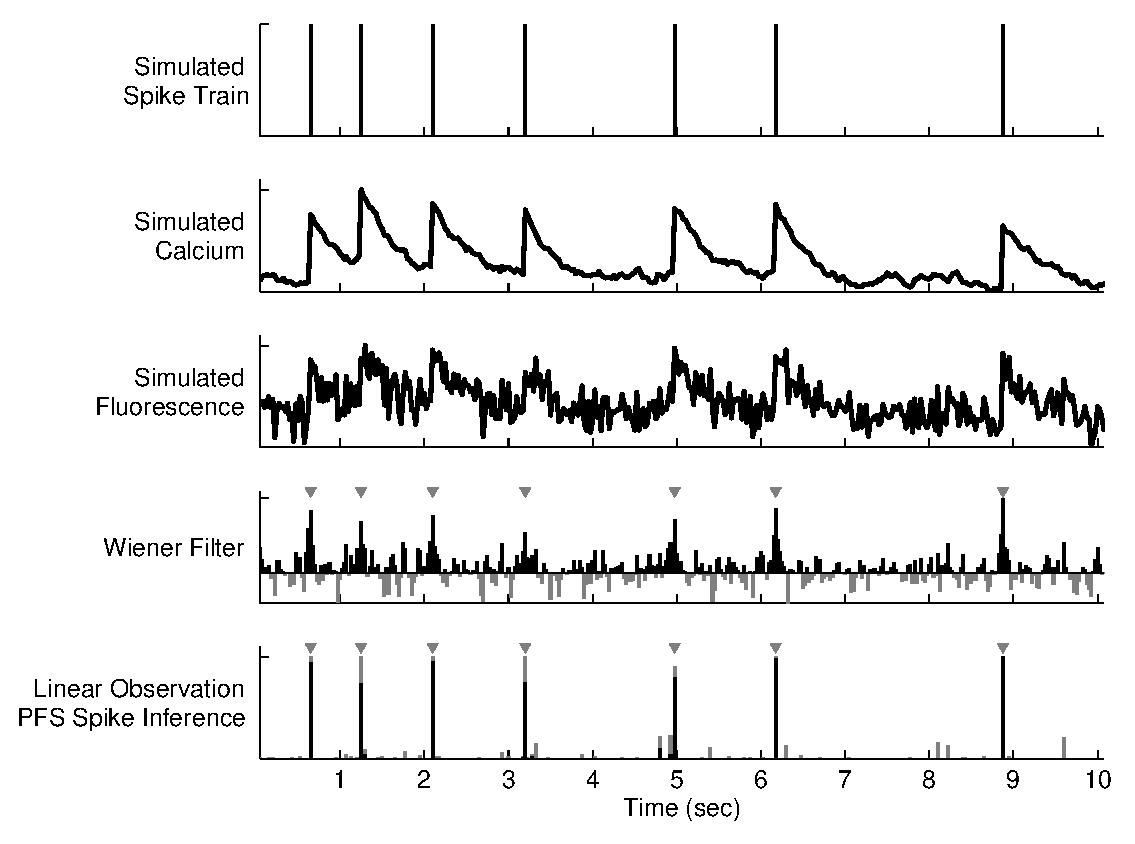
\includegraphics[width=1.0\linewidth]{NoisySim_bw}
\caption{Main result}  \label{fig:noisy}
\end{figure}

\clearpage \newpage
\begin{figure}
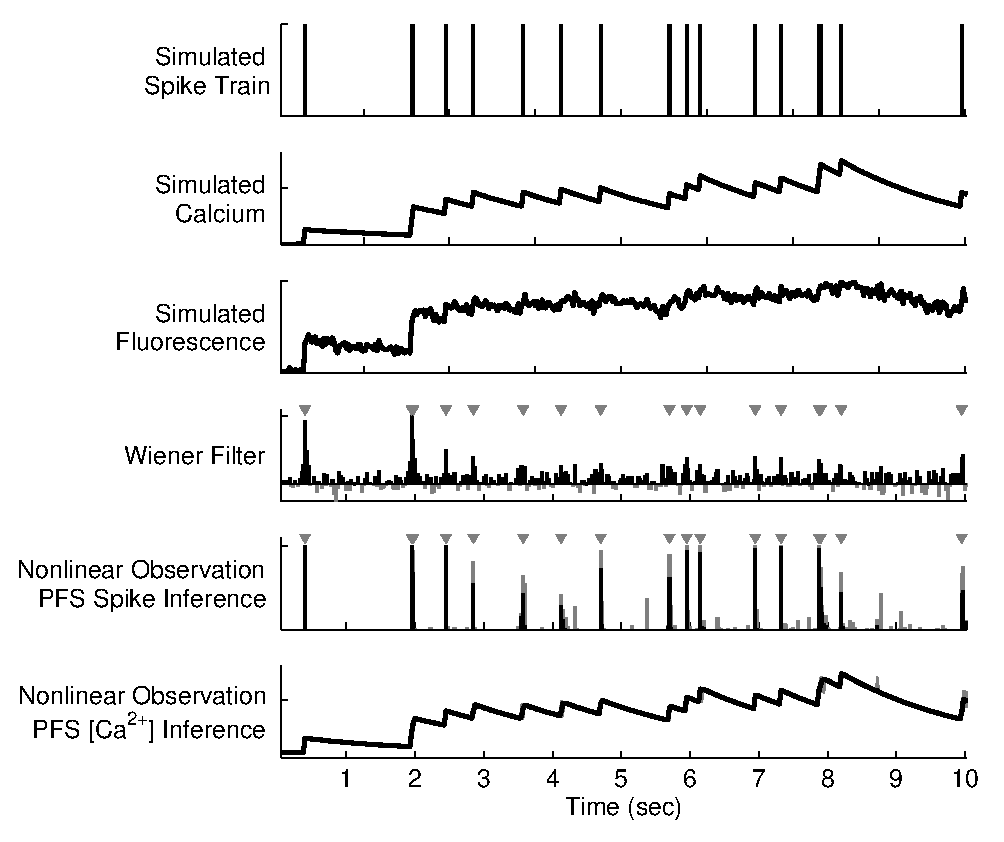
\includegraphics[width=1.0\linewidth]{SaturSim_bw}
\caption{Saturated simulation} \label{fig:SaturSim}
\end{figure}

\clearpage \newpage
\begin{figure}
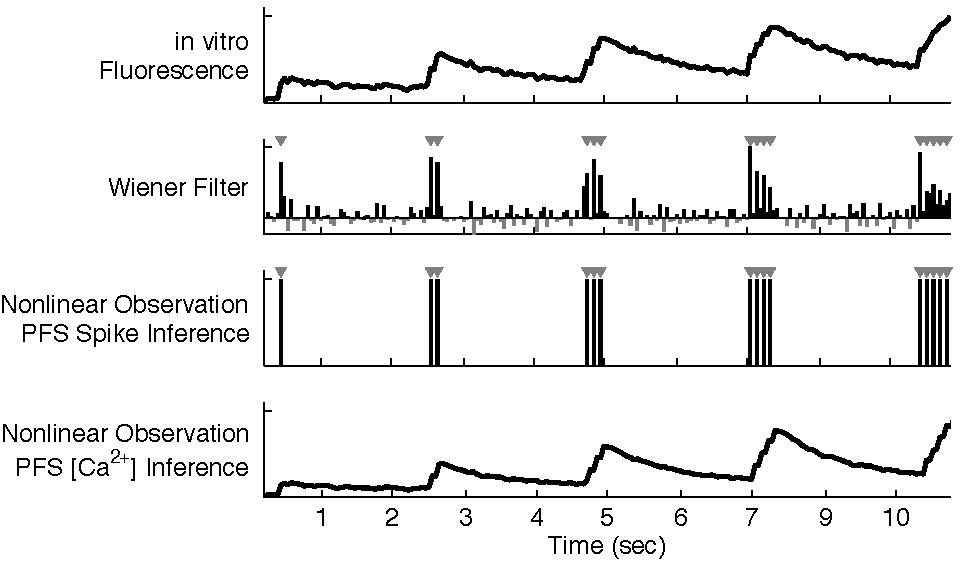
\includegraphics[width=1.0\linewidth]{BurstData_bw}
\caption{In vitro bursts} \label{fig:BurstData}
\end{figure}

\clearpage \newpage
\begin{figure}
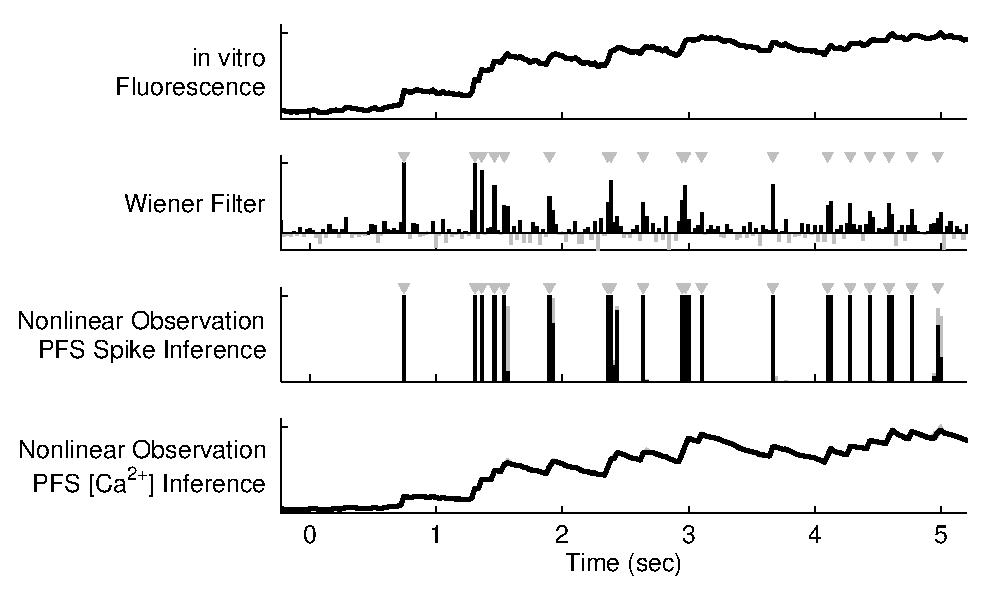
\includegraphics[width=1.0\linewidth]{SaturData_bw}
\caption{Real data saturation} \label{fig:SaturData}
\end{figure}

\clearpage \newpage
\begin{figure}
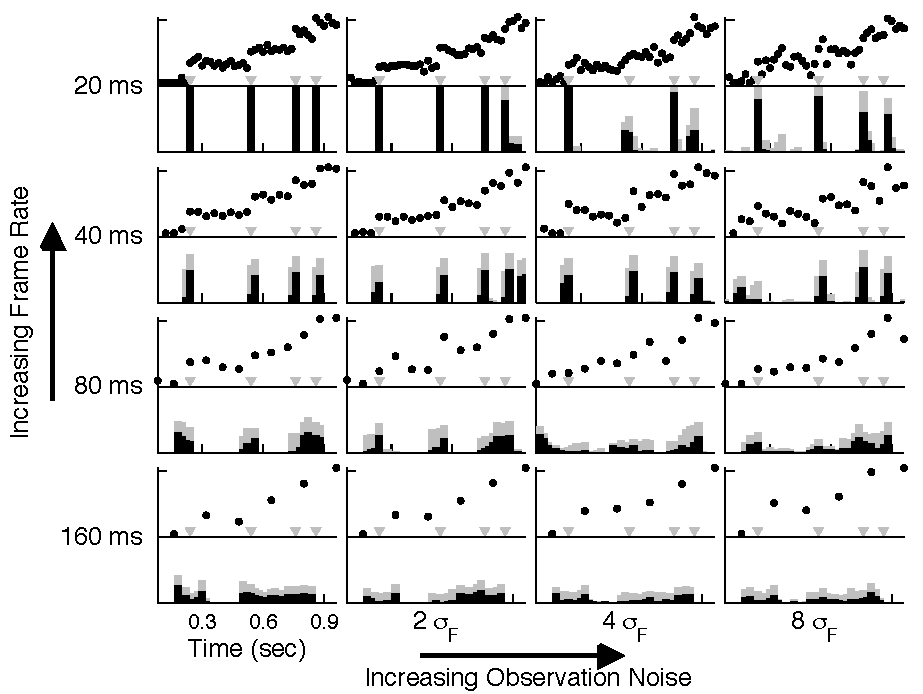
\includegraphics[width=1.0\linewidth]{ArraySim_bw}
\caption{Array of inferences} \label{fig:array}
\end{figure}

\clearpage \newpage
\begin{figure}
\begin{centering}
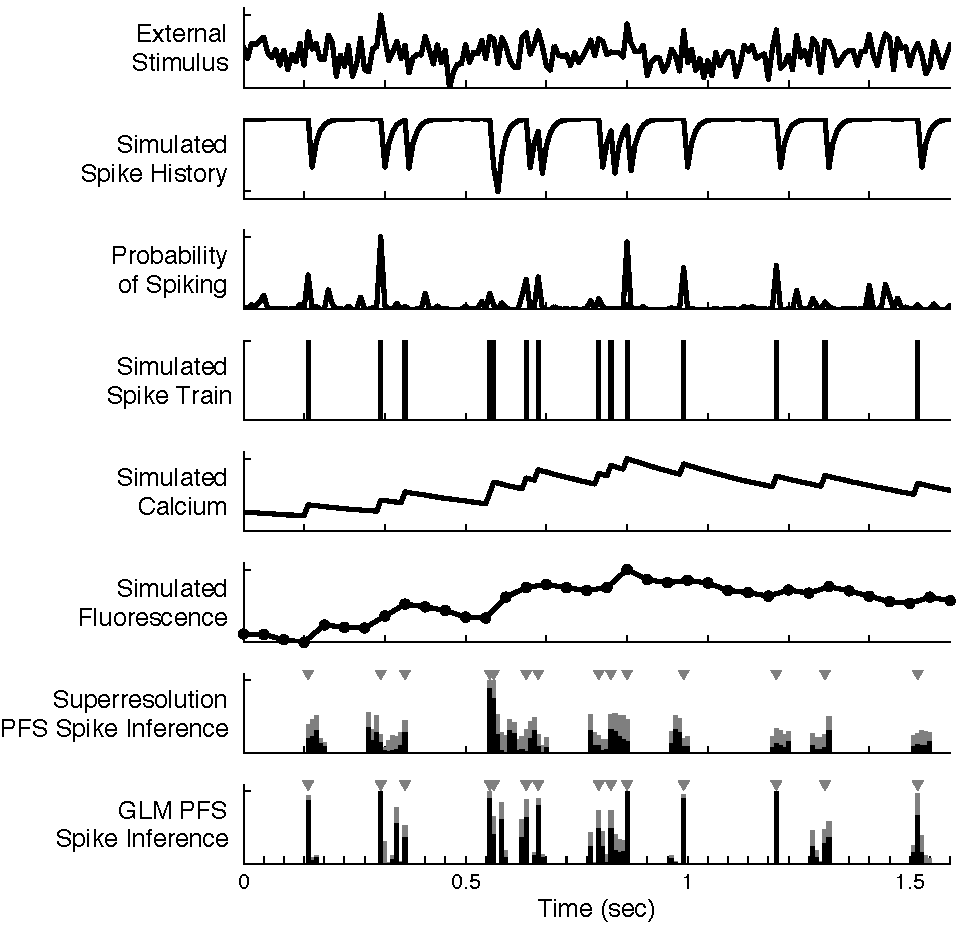
\includegraphics[width=1\linewidth]{StimSim_bw}
\end{centering}
\caption{Generalized Linear Model Particle Filter Smoother} \label{fig:StimSim}
\end{figure}

\clearpage \newpage
\begin{figure}
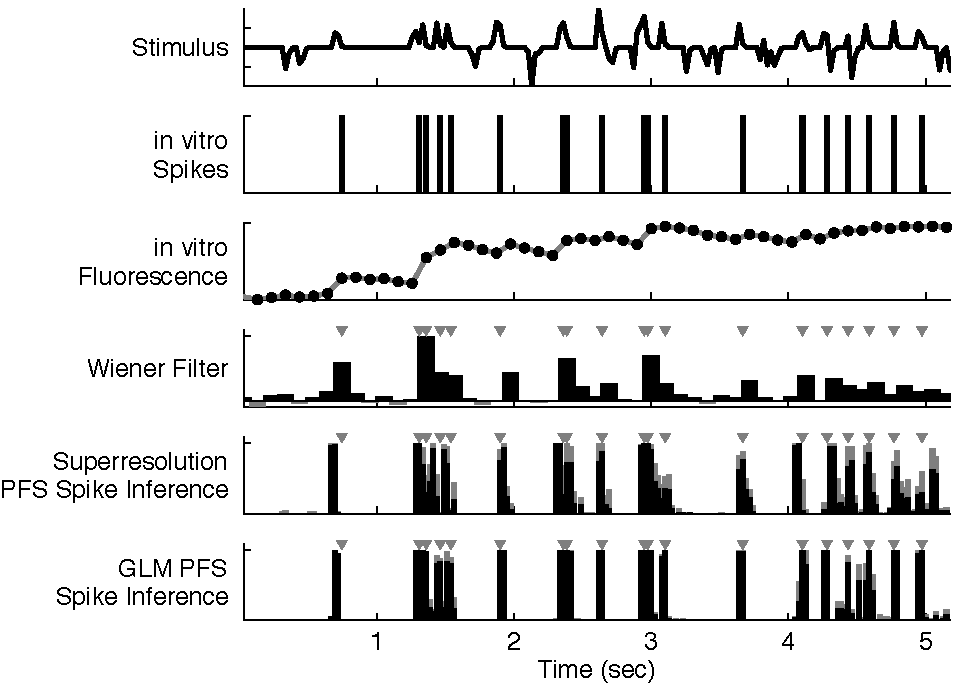
\includegraphics[width=1.0\linewidth]{StimData_bw}
\caption{In vitro data superresolution} \label{fig:real}
\end{figure}

\clearpage \newpage
\begin{figure}
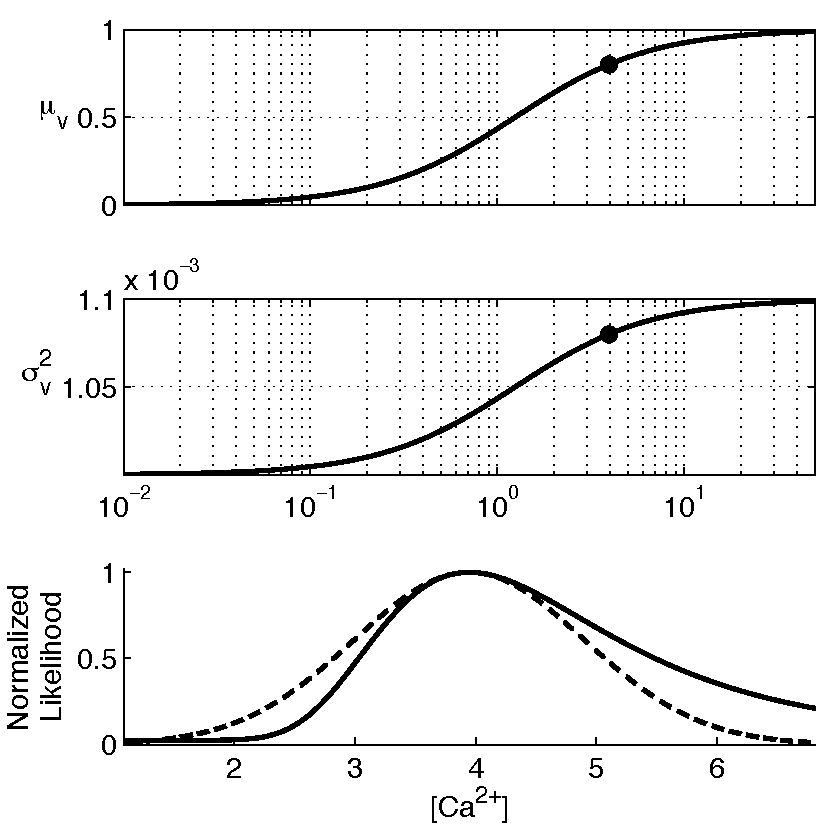
\includegraphics[width=\linewidth]{ca_nonlin}
\caption{Laplace approximation of observation distribution} \label{fig:ca_nonlin}
\end{figure}

\clearpage \newpage
\begin{figure}
\centering 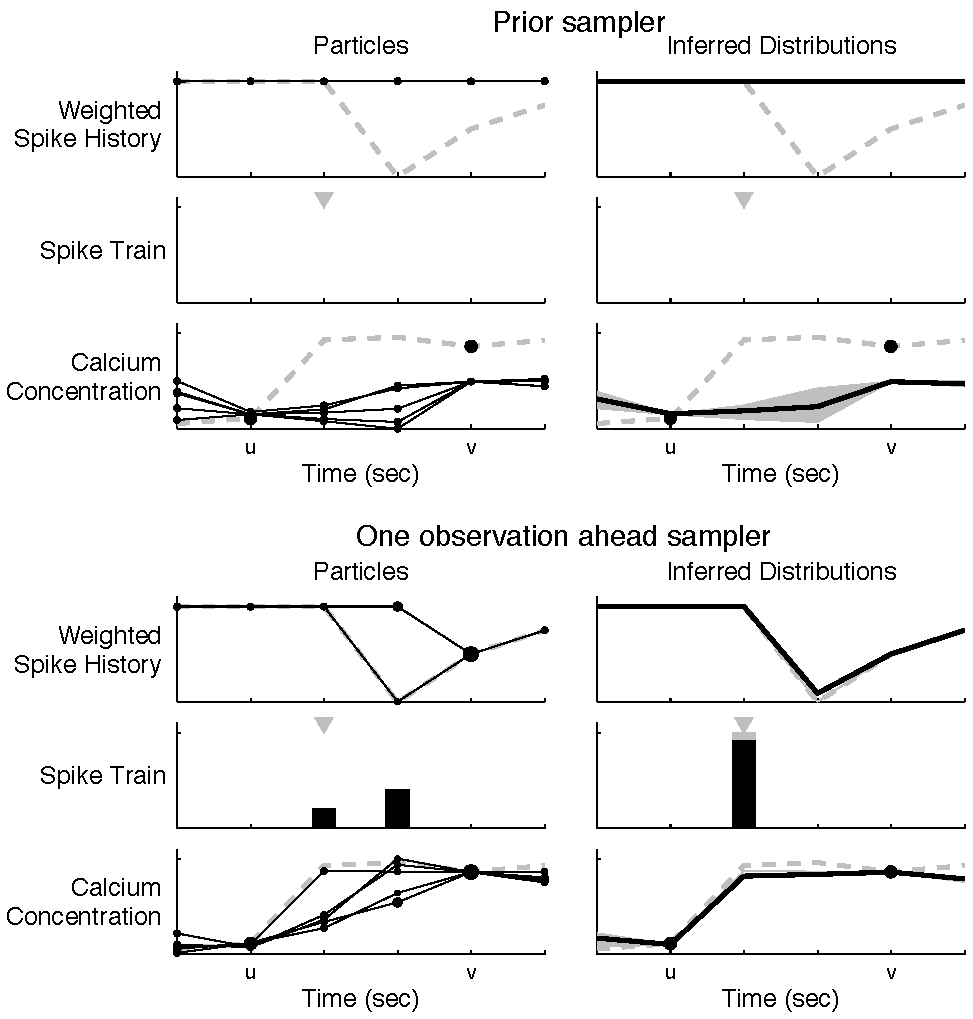
\includegraphics[width=1\linewidth]{SimSampl_bw}
\caption{Sampling strategies} \label{fig:sampl}
\end{figure}

\clearpage \newpage
\begin{figure}
\centering
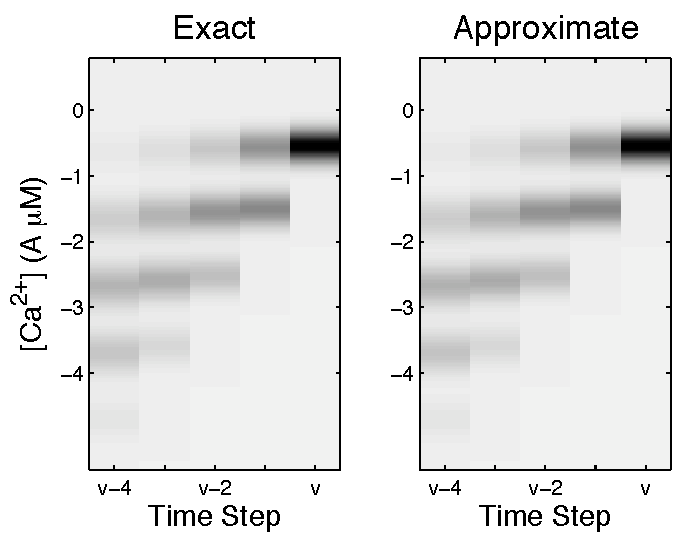
\includegraphics[width=0.5\linewidth]{PFapprox2}
\caption{Mixture approximation} \label{fig:pf2}
\end{figure}
\end{document} 

